\documentclass[12pt,a4paper]{report}
\usepackage{xcolor}
% ---------------- Packages ----------------
\usepackage{graphicx}
\usepackage{geometry}
\usepackage{setspace}
\usepackage{tocloft}
\usepackage{enumitem}
\usepackage{needspace}
\usepackage{pdfpages}
\usepackage{titlesec}
\usepackage{fancyhdr}
\usepackage{tikz}
\usetikzlibrary{shapes.geometric, arrows.meta, positioning, calc, fit, backgrounds}

% ---------------- Page Setup ----------------
\geometry{
left=1.25in,
right=1in,
top=1in,
bottom=1in
}

\onehalfspacing
\setlength{\parindent}{0pt}
\setlength{\parskip}{8pt}
\setlength{\headheight}{15pt}

% ---------------- Custom Font Command ----------------
\newcommand{\headingSixteen}[1]{{\fontsize{16pt}{18pt}\selectfont\textbf{#1}}}
\newcommand{\headingFourteen}[1]{{\fontsize{14pt}{16pt}\selectfont\textbf{#1}}}

% ---------------- Table of Contents Formatting ----------------

\renewcommand{\contentsname}{TABLE OF CONTENTS}

\setlength{\cftbeforetoctitleskip}{17pt}
\setlength{\cftaftertoctitleskip}{20pt}

\setlength{\cftchapindent}{0pt}
\setlength{\cftsecindent}{1.5em}
\setlength{\cftsubsecindent}{3.5em}

\renewcommand{\cftchapfont}{\bfseries}
\renewcommand{\cftchappagefont}{\bfseries}

\renewcommand{\cftdotsep}{1}
\setlength{\cftbeforechapskip}{6pt}

\makeatletter
\renewcommand{\@cftmaketoctitle}{%
\chapter*{%
\centering
\fontsize{14pt}{16pt}\selectfont
\textbf{TABLE OF CONTENTS}
}
}
\makeatother

% ---------------- Section Formatting ----------------
\titlespacing*{\section}{0pt}{14pt}{10pt}
\titlespacing*{\subsection}{0pt}{12pt}{8pt}

\titleformat{\section}
{\bfseries\fontsize{14pt}{16pt}\selectfont}
{\thesection}

{1em}
{}

\titleformat{\subsection}
{\bfseries\fontsize{12pt}{14pt}\selectfont}
{\thesubsection}
{1em}
{}

% ---------------- Header & Footer ----------------
\fancypagestyle{maincontent}{
\fancyhf{}
\fancyhead[R]{\small Tourism Promotion Website}
\fancyfoot[L]{\small Saintgits College of Engineering (Autonomous)}
\fancyfoot[R]{\small \thepage}
\renewcommand{\headrulewidth}{0.4pt}
\renewcommand{\footrulewidth}{0.4pt}
}

% Style for Chapter Title Pages (NO header, NO footer)
\fancypagestyle{plain}{
\fancyhf{}
\renewcommand{\headrulewidth}{0pt}
\renewcommand{\footrulewidth}{0pt}
}

% ---------------- Bibliography Spacing ----------------
\makeatletter
\renewenvironment{thebibliography}[1]
{\section*{}\@mkboth{}{}%
\list{\@biblabel{\@arabic\c@enumiv}}%
{\settowidth\labelwidth{\@biblabel{#1}}%
\leftmargin\labelwidth
\advance\leftmargin\labelsep
\itemsep=0.6\baselineskip
\usecounter{enumiv}%
\let\p@enumiv\@empty
\renewcommand\theenumiv{\@arabic\c@enumiv}}%

\sloppy}
{\endlist}
\makeatother

% =====================================================
\begin{document}

% ===================== PAGE 1 : TITLE PAGE =====================
\thispagestyle{empty}

\begin{center}

\vspace*{0.3cm}
\headingSixteen{PERSONALIZED LEARNING TRACKS (TRACK 3)}\\[0.35cm]
\headingSixteen{SDG PROJECT REPORT}\\[0.25cm]
\headingFourteen{ON}\\[0.25cm]

\headingSixteen
{\textcolor{blue}{TOURISM PROMOTION WEBSITE}}\\[0.6cm]

\headingFourteen{Submitted By}\\[0.15cm]

\headingFourteen
{\textcolor{blue}
{SOJU YOHANNAN - MGP25MCA-2058}}\\[0.6cm]

\headingFourteen{To}\\[0.15cm]

\textit{the APJ Abdul Kalam Technological University in partial}\\
\textit{fulfillment of the requirements for the award of the degree of}\\[0.4cm]

\headingFourteen{MASTER OF COMPUTER APPLICATIONS}\\[0.6cm]

\headingFourteen{Under the guidance of}\\[0.2cm]

\headingFourteen
{\textcolor{blue}{Dr. Amrita Priya K}}\\
\headingFourteen
{\textcolor{blue}{Assistant Professor}}\\[0.8cm]

\includegraphics[width=3.8cm]{Saintgits logo New.png}\\[0.8cm]

\headingFourteen{DEPARTMENT OF COMPUTER APPLICATIONS}\\[0.15cm]

\headingFourteen{SAINTGITS COLLEGE OF ENGINEERING (AUTONOMOUS)}\\

\headingFourteen{Pathamuttom, Kottayam, Kerala – 686532}\\[0.45cm]

\textit{(Approved by AICTE and affiliated to APJ Abdul Kalam Technological University)}
\\[0.99cm]

\headingSixteen{AUGUST 2026}

\end{center}
% ===================== PAGE 2 : BONAFIDE =====================
\newpage
\thispagestyle{empty}

\begin{center}
\fontsize{16pt}{18pt}\selectfont
\textbf{SAINTGITS COLLEGE OF ENGINEERING (AUTONOMOUS)}\\
Kottukulam Hills, Pathamuttom, Kottayam, Kerala – 686532

\end{center}

\vspace{0.2cm}

\begin{center}
\includegraphics[width=4.5cm]{Saintgits logo New.png}
\end{center}

\vspace{0.1cm}

\begin{center}
\fontsize{16pt}{18pt}\selectfont
\textbf{BONAFIDE CERTIFICATE}
\end{center}

\vspace{0.2cm}

Certified that the report entitled \textbf{“Tourism Promotion Website”} submitted by \textbf{“SOJU YOHANNAN - MGP25MCA-2058”} to the APJ
Abdul Kalam Technological University in partial fulfillment of the requirements for the award of the
Degree of \textbf{Master of Computer Applications} is a bonafide record of the \textbf{Social
Immersion Sustainable Development Goals(SDG)} project work carried out by him / her under our
guidance and supervision. This report in any form has not been submitted to any other University or
Institute for any purpose.

\vspace{2.2cm}

\noindent
\begin{minipage}[t]{0.45\textwidth}
\raggedright
\textbf{Dr.Amrita Priya K}\\
Internal Guide
\end{minipage}

\hfill
\begin{minipage}[t]{0.45\textwidth}
\raggedleft
\textbf{Ms. Ankitha Philip}\\
SDG Project Coordinator
\end{minipage}

\vspace{2.5cm}

\noindent
\begin{center}
\begin{minipage}{0.45\textwidth}
\centering
\textbf{Dr. Rani Saritha R}\\
Head of the Department
\end{minipage}
\end{center}
\vspace{1.8cm}

% ===================== PAGE 3 : ACKNOWLEDGEMENT =====================
\newpage
\thispagestyle{empty}

\begin{center}
\fontsize{16pt}{18pt}\selectfont
\textbf{ACKNOWLEDGEMENT}
\end{center}

\vspace{1cm}

At the outset, I thank the Lord Almighty for His abundant grace, strength and hope to make our
endeavour a success. I express my deep-felt gratitude to \textbf{Dr. Sudha T}, Principal, Saintgits
College of Engineering (Autonomous), for her warm support with regard to the work and to the
management for providing the facilities required.

I would like to place my deep sense of gratitude to \textbf{Prof. Mini Punnoose},\linebreak Director
MCA, Department of Computer Applications, Saintgits College of Engineering (Autonomous), for her
constant encouragement.I express my gratitude to \linebreak\textbf{Dr. Rani Saritha R}, Head of the
Department, Department of Computer Applications, Saintgits College of Engineering (Autonomous),
for her support and guidance.

I am profoundly grateful to \textbf{Dr.Amrita Priya K}, my SDG Project Guide and\linebreak\textbf{Ms.
Ankitha Philip}, the SDG Project Coordinator, for their valuable guidance, help, suggestions and
assessment.

Furthermore, I would like to thank all others, especially my parents and numerous friends. This
project report would not have been a success without their inspiration, valuable suggestions and
moral support from them throughout its course.

\vspace{2cm}

\begin{flushright}
\textbf{Soju Yohannan}
\end{flushright}

% ===================== PAGE 4 : ABSTRACT =====================
\newpage
\thispagestyle{empty}

\begin{center}
\fontsize{16pt}{18pt}\selectfont
\textbf{ABSTRACT}
\end{center}

\vspace{1cm}
\textcolor{red}{\textbf{Tourism Promotion Website }}\\
#

The Tourism Promotion Website is a comprehensive digital platform developed to stimulate local economic growth and sustainable tourism. The platform serves a dual purpose: providing tourists with an engaging, interactive interface to discover heritage destinations and book curated travel packages, while simultaneously offering a dedicated marketplace for local service providers—such as hoteliers, tour guides, restaurant owners, and artisans—to register and promote their businesses directly to global consumers.

Built upon a robust, role-based architecture (Admin, Tourist, and Service Provider) using Node.js, Express.js, and a MySQL relational database, the system ensures secure, isolated access to modular functionalities through JSON Web Token (JWT) authentication. Administrators maintain overarching control over destinations, packages, and platform governance. Service providers are equipped with a specialized dashboard to manage their specific service listings and analyze tourist interest. Tourists enjoy a seamless, secure experience for exploring locations, managing booking itineraries, and contributing community reviews.

The platform also promotes local culture, traditional products, and lesser-known destinations, helping distribute tourism benefits among local communities. By connecting tourists directly with local businesses, the system creates new digital opportunities for small-scale service providers and supports sustainable economic development.

The project aligns with key **Sustainable Development Goals (SDGs), particularly SDG 8 (Decent Work and Economic Growth),  by promoting local entrepreneurship, cultural heritage, and responsible tourism practices.

Ultimately, the project leverages modern web technologies to bridge the gap between travelers and local communities, fostering inclusive economic opportunities, supporting small businesses, and preserving cultural heritage through accessible digital infrastructure.
.
% ===================== TABLE OF CONTENTS =====================

\clearpage
\pagenumbering{gobble} % &lt;-- completely removes page number
\pagenumbering{gobble} % <-- completely removes page number
\pagestyle{empty} % <-- removes header & footer
\tableofcontents

\clearpage

\pagenumbering{arabic} % <-- restores numbering
\pagestyle{maincontent} % <-- restores header/footer

% ===================== CHAPTERS =====================
% ===================== CHAPTER 1 : INTRODUCTION =====================
\chapter{INTRODUCTION}

\section{Project Overview}

The \textbf{Tourism Promotion Website} is a full-stack web application designed to promote sustainable tourism by connecting tourists with local service providers across popular Indian destinations. The platform operates as a digital marketplace where tourists can explore heritage sites, book curated travel packages, access local services, and contribute community-driven reviews---while simultaneously empowering local businesses such as hotels, restaurants, tour guides, transport operators, and handicraft vendors to register, list, and manage their services online.

The project was developed as part of the \textbf{Social Immersion Sustainable Development Goals (SDG)} initiative under Personalized Learning Tracks (Track 3). It addresses the need for a centralized digital platform that bridges the gap between travelers and local communities, enabling inclusive economic participation and cultural preservation through technology.

The application features a role-based architecture with three distinct user roles:
\begin{itemize}[leftmargin=2em]
    \item \textbf{Administrator:} Manages destinations, travel packages, events, user accounts, service provider approvals, and platform-wide analytics.
    \item \textbf{Tourist (User):} Browses destinations, books packages, accesses local services, manages wishlists and itineraries, writes reviews, and makes secure payments.
    \item \textbf{Service Provider:} Registers a business profile, lists services linked to specific destinations, tracks bookings, and manages service offerings through a dedicated dashboard.
\end{itemize}

The system is built using \textbf{Node.js} and \textbf{Express.js} on the server side, with a \textbf{MySQL} relational database for data persistence. The front end uses \textbf{HTML5, CSS3, JavaScript}, and \textbf{Bootstrap 5} for a responsive, mobile-friendly user interface. Authentication is handled through \textbf{JSON Web Tokens (JWT)} combined with server-side session management for secure, role-isolated access control.

\section{Objectives}

The primary objectives of the Tourism Promotion Website are:

\begin{enumerate}[leftmargin=2em]
    \item To design and develop a comprehensive web-based tourism marketplace that facilitates discovery of tourist destinations, booking of travel packages, and access to local services.
    \item To create a role-based access control system with separate dashboards and functionalities for administrators, tourists, and local service providers.
    \item To provide local service providers---including hoteliers, tour guides, restaurant owners, transport operators, and artisans---a digital platform to register, list, and promote their businesses directly to tourists.
    \item To implement secure user authentication and session management using JWT tokens and Express sessions.
    \item To build an administrative control panel for managing destinations, packages, events, user governance, provider approvals, and platform analytics.
    \item To integrate a booking and payment management system with status tracking (Pending, Confirmed, Completed, Cancelled) and payment processing.
    \item To support community-driven engagement through a reviews and ratings system for destinations, services, and packages.
    \item To implement a wishlist feature enabling tourists to save and organize preferred destinations for future travel planning.
    \item To promote the goals of \textbf{SDG 8 (Decent Work and Economic Growth)} by creating digital economic opportunities for small-scale local service providers and supporting sustainable tourism practices.
    \item To design a responsive, visually appealing user interface with modern design elements including dark/light theme toggling, glassmorphism, and smooth animations.
\end{enumerate}

\section{Scope of the Project}

The scope of the Tourism Promotion Website encompasses the following functional and technical areas:

\needspace{5\baselineskip}
\textbf{Functional Scope:}
\begin{itemize}[leftmargin=2em]
    \item \textbf{Destination Management:} CRUD operations for tourist destinations with support for categories (Hill Station, Beach, Heritage, Wildlife, Pilgrimage), image galleries, seasonal information, budget ranges, nearby attractions, and featured destination tagging.
    \item \textbf{Travel Package Management:} Creation and management of curated multi-day travel packages linked to specific destinations, with pricing, descriptions, and itinerary details.
    \item \textbf{Local Service Marketplace:} A service listing system supporting multiple service types (Hotels, Guides, Taxis, Restaurants, Handicrafts) with fixed and per-kilometer pricing models, provider profiles, and admin approval workflows.
    \item \textbf{Booking System:} End-to-end booking lifecycle management including booking creation, status updates, guest count, travel date selection, distance-based pricing calculation, and special request handling.
    \item \textbf{Payment Processing:} Simulated payment gateway with card-based payment, unique reference generation, and payment status tracking (Unpaid, Paid, Refunded).
    \item \textbf{Reviews and Ratings:} User-submitted reviews for destinations, services, and packages with star ratings and textual comments.
    \item \textbf{Wishlist Management:} Personal wishlist functionality for registered tourists to bookmark destinations.
    \item \textbf{Notification System:} In-app notifications for admin alerts (new provider registrations, booking updates) and user-facing notifications.
    \item \textbf{Analytics Dashboard:} Administrative analytics providing insights into booking trends, revenue metrics, popular destinations, and user activity.
    \item \textbf{Event Management:} Listing and promotion of local cultural events, festivals, and community activities tied to tourist destinations.
\end{itemize}

\needspace{5\baselineskip}
\textbf{Technical Scope:}
\begin{itemize}[leftmargin=2em]
    \item Full-stack web application using Node.js, Express.js, MySQL, HTML5, CSS3, JavaScript, and Bootstrap 5.
    \item RESTful API design with modular route handling for authentication, destinations, bookings, services, reviews, events, packages, providers, notifications, analytics, uploads, wishlists, and payments.
    \item Role-based middleware for access control with JWT verification.
    \item File upload handling using Multer for service provider images and destination galleries.
    \item Responsive design supporting desktop, tablet, and mobile viewports.
    \item Session-based route protection for dashboard directories.
\end{itemize}

\needspace{5\baselineskip}
\textbf{Limitations of Scope:}
\begin{itemize}[leftmargin=2em]
    \item The payment system uses a simulated gateway and does not integrate with live payment processors such as Razorpay or Stripe.
    \item The application is designed for single-server deployment and does not include distributed system or microservices architecture.
    \item Real-time features such as live chat or push notifications are not implemented in the current version.
    \item Multi-language support and advanced accessibility features are planned for future iterations.
\end{itemize}

% ===================== CHAPTER 2 : SUSTAINABLE DEVELOPMENT GOAL =====================
\chapter{SUSTAINABLE DEVELOPMENT GOAL}

\section{Overview of Sustainable Development Goal}

The \textbf{Sustainable Development Goals (SDGs)}, also known as the Global Goals, are a collection of 17 interlinked objectives adopted by all United Nations Member States in 2015 as part of the \textit{2030 Agenda for Sustainable Development}. These goals serve as a universal call to action to end poverty, protect the planet, and ensure that all people enjoy peace and prosperity by 2030.

The SDGs address a broad range of global challenges including inequality, climate change, environmental degradation, peace, and justice. Each goal has specific targets and indicators to measure progress. The goals are designed to be interconnected---progress in one area often supports progress in others, recognizing that development must balance social, economic, and environmental sustainability.

The 17 SDGs are:
\begin{enumerate}[leftmargin=2em]
    \item No Poverty
    \item Zero Hunger
    \item Good Health and Well-being
    \item Quality Education
    \item Gender Equality
    \item Clean Water and Sanitation
    \item Affordable and Clean Energy
    \item Decent Work and Economic Growth
    \item Industry, Innovation and Infrastructure
    \item Reduced Inequalities
    \item Sustainable Cities and Communities
    \item Responsible Consumption and Production
    \item Climate Action
    \item Life Below Water
    \item Life on Land
    \item Peace, Justice and Strong Institutions
    \item Partnerships for the Goals
\end{enumerate}

In the context of this project, the focus is primarily on \textbf{SDG 8: Decent Work and Economic Growth}, with secondary alignment to SDG 9 (Industry, Innovation and Infrastructure) and SDG 11 (Sustainable Cities and Communities).

\section{Selected SDG(s)}

The Tourism Promotion Website directly aligns with:

\textbf{SDG 8: Decent Work and Economic Growth}

\textit{``Promote sustained, inclusive and sustainable economic growth, full and productive employment and decent work for all.''}

Specific targets addressed include:

\begin{itemize}[leftmargin=2em]
    \item \textbf{Target 8.3:} Promote development-oriented policies that support productive activities, decent job creation, entrepreneurship, creativity and innovation, and encourage the formalization and growth of micro-, small- and medium-sized enterprises.
    \item \textbf{Target 8.9:} By 2030, devise and implement policies to promote sustainable tourism that creates jobs and promotes local culture and products.
    \item \textbf{Target 8.10:} Strengthen the capacity of domestic financial institutions to encourage and expand access to banking, insurance and financial services for all.
\end{itemize}

\textbf{Secondary SDG Alignment:}
\begin{itemize}[leftmargin=2em]
    \item \textbf{SDG 9 (Industry, Innovation and Infrastructure):} The project uses modern web technologies and digital infrastructure to create an innovative marketplace connecting tourists with local service providers.
    \item \textbf{SDG 11 (Sustainable Cities and Communities):} By promoting heritage sites, cultural events, and local communities, the platform supports the preservation of cultural and natural heritage.
\end{itemize}

\section{Problem Addressed}

The tourism industry in India, while being one of the largest contributors to the national economy, faces several challenges that disproportionately affect local communities and small-scale service providers:

\begin{enumerate}[leftmargin=2em]
    \item \textbf{Digital Divide:} Many local service providers---including small hoteliers, independent tour guides, local transport operators, restaurant owners, and artisans---lack the technical expertise and financial resources to establish an online presence. They remain invisible to the digital-savvy tourist who relies on online platforms for travel planning.

    \item \textbf{Dominance of Large Aggregators:} Existing tourism platforms (such as MakeMyTrip, Booking.com, and TripAdvisor) are dominated by large hospitality chains and established businesses. Small, community-based service providers are often excluded from these platforms due to high commission structures, complex onboarding processes, and visibility algorithms that favor larger operators.

    \item \textbf{Fragmented Information:} Tourists seeking authentic, local experiences often struggle to find consolidated information about local services, cultural events, heritage sites, and community-based tourism options. Information is scattered across multiple sources, making trip planning inefficient.

    \item \textbf{Limited Economic Distribution:} Tourism revenue in many destinations is concentrated among a few large operators, while local communities that form the cultural backbone of these destinations receive minimal economic benefit.

    \item \textbf{Lack of Direct Connection:} There is no direct digital channel connecting tourists with local service providers. Intermediaries often control the interaction, reducing the provider's margin and the tourist's ability to access authentic experiences.
\end{enumerate}

\section{Contribution of the Proposed Project towards the SDG(s)}

The Tourism Promotion Website addresses the identified problems through the following contributions:

\begin{enumerate}[leftmargin=2em]
    \item \textbf{Digital Marketplace for Local Providers:} The platform provides a free, accessible digital marketplace where local service providers can register, create business profiles, list their services (hotels, restaurants, guides, transport, handicrafts), and directly reach tourists without intermediaries. The admin approval workflow ensures quality control while keeping the barrier to entry low.

    \item \textbf{Promoting Local Entrepreneurship:} By providing dedicated provider dashboards with service management tools, the platform empowers local entrepreneurs to manage their businesses digitally, track tourist interest, and grow their customer base. This directly supports \textbf{SDG Target 8.3} on entrepreneurship and small enterprise formalization.

    \item \textbf{Sustainable Tourism Promotion:} The platform curates and promotes heritage destinations, cultural events, local cuisine, and traditional crafts alongside mainstream tourist attractions. This aligns with \textbf{SDG Target 8.9} on promoting sustainable tourism that supports local culture and products.

    \item \textbf{Economic Inclusion:} The role-based architecture ensures that local service providers have equal visibility and tools as any other participant on the platform. The system enables direct transactions between tourists and providers, maximizing revenue retention for local communities.

    \item \textbf{Community Engagement:} Features such as community reviews, event listings, and destination highlights create a feedback loop that encourages tourists to engage with local culture and services, driving repeat visits and sustained economic activity.

    \item \textbf{Cultural Preservation:} By highlighting heritage destinations, traditional crafts, local festivals, and cultural walks, the platform contributes to the preservation and promotion of India's diverse cultural heritage.
\end{enumerate}

\section{Expected Social and Environmental Impact}

\textbf{Social Impact:}
\begin{itemize}[leftmargin=2em]
    \item \textbf{Employment Generation:} The platform creates digital economic opportunities for local service providers, potentially generating direct and indirect employment in tourism-dependent communities.
    \item \textbf{Skill Development:} Service providers using the platform gain digital literacy skills through the process of registering, managing profiles, listing services, and interacting with a web-based dashboard.
    \item \textbf{Community Empowerment:} Local communities gain a voice and visibility in the tourism ecosystem, enabling them to benefit directly from tourist spending rather than through intermediaries.
    \item \textbf{Cultural Exchange:} The platform facilitates meaningful cultural exchange between tourists and local communities through features like heritage walks, local food experiences, craft markets, and cultural events.
    \item \textbf{Inclusive Growth:} By providing equal access to the platform for all service providers regardless of size, the system promotes inclusive economic growth in line with SDG 8.
\end{itemize}

\textbf{Environmental Impact:}
\begin{itemize}[leftmargin=2em]
    \item \textbf{Promoting Responsible Tourism:} By highlighting eco-friendly destinations, nature trails, and wildlife conservation areas, the platform encourages responsible tourism practices.
    \item \textbf{Reducing Over-tourism:} The platform promotes lesser-known destinations alongside popular ones, helping distribute tourist traffic more evenly and reducing environmental pressure on over-visited locations.
    \item \textbf{Digital-First Approach:} The paperless, digital nature of the booking, payment, and review systems reduces the environmental footprint associated with traditional tourism operations.
    \item \textbf{Community-Based Conservation:} By linking tourism revenue to local communities, the platform creates economic incentives for communities to preserve their natural and cultural environments.
\end{itemize}

% ===================== CHAPTER 3 : REQUIREMENT ANALYSIS =====================
\chapter{REQUIREMENT ANALYSIS}

\section{Existing System}

The existing landscape of tourism-related digital platforms in India is dominated by large commercial aggregators such as MakeMyTrip, Booking.com, Goibibo, and TripAdvisor. While these platforms provide extensive listings for hotels, flights, and popular tourist packages, they exhibit several limitations from the perspective of local community empowerment and sustainable tourism:

\begin{itemize}[leftmargin=2em]
    \item \textbf{High Barriers to Entry:} Small-scale local service providers such as independent guides, homestay operators, local transport providers, and artisans face significant barriers to listing on established platforms. These include high commission rates (15--25\%), complex registration processes, and stringent listing requirements.
    \item \textbf{Lack of Provider Dashboards:} Most existing platforms do not provide small providers with meaningful tools to manage their services, track engagement, or analyze tourist interest. The focus is on large hospitality chains with dedicated account management.
    \item \textbf{No SDG Alignment:} Existing commercial platforms are profit-driven and do not explicitly aim to promote sustainable development goals, local entrepreneurship, or cultural preservation.
    \item \textbf{Fragmented User Experience:} Tourists seeking authentic local experiences must navigate multiple platforms and offline sources to find information about local guides, cultural events, handicraft markets, and community-based services.
    \item \textbf{Limited Community Engagement:} Review systems on existing platforms primarily focus on large hotels and restaurants, offering minimal visibility for small, community-based services.
    \item \textbf{No Role-Based Architecture:} Existing platforms typically operate on a two-tier model (platform and user), lacking the three-tier role-based system (Admin, Tourist, Service Provider) needed for community-centric tourism promotion.
\end{itemize}

\textbf{Limitations of the Existing System:}
\begin{enumerate}[leftmargin=2em]
    \item Local service providers are excluded from mainstream digital tourism platforms.
    \item There is no dedicated marketplace for community-based tourism services.
    \item Tourism revenue is concentrated among large operators, with minimal trickle-down to local economies.
    \item Cultural heritage, local events, and artisan products lack digital promotion channels.
    \item No existing platform integrates SDG-aligned features for sustainable tourism.
\end{enumerate}

\section{Proposed System}

The \textbf{Tourism Promotion Website} is a purpose-built, full-stack web application that addresses the shortcomings of existing systems by providing:

\begin{itemize}[leftmargin=2em]
    \item \textbf{Three-Tier Role-Based Architecture:} The system implements three distinct user roles---Administrator, Tourist, and Service Provider---each with dedicated dashboards, permissions, and functionalities. This ensures that local service providers have first-class access to the platform alongside tourists and administrators.

    \item \textbf{Free Digital Marketplace:} Service providers can register and list their services at no cost, with a simple admin approval workflow that ensures quality while keeping the onboarding process accessible.

    \item \textbf{Integrated Tourism Ecosystem:} The platform integrates destination discovery, package booking, local service access, event listings, community reviews, wishlists, and payments into a single, cohesive user experience.

    \item \textbf{Provider Empowerment Tools:} Service providers receive a dedicated dashboard to manage service listings, track bookings, update business profiles, and monitor tourist engagement.

    \item \textbf{Admin Governance:} Administrators have full control over platform content, user management, provider approvals, analytics, and quality assurance through a comprehensive admin dashboard.

    \item \textbf{SDG-Aligned Design:} The platform is explicitly designed to promote SDG 8 (Decent Work and Economic Growth) through digital entrepreneurship enablement, local culture promotion, and inclusive tourism practices.

    \item \textbf{Modern, Responsive UI:} The front end uses Bootstrap 5 with custom CSS, glassmorphism effects, dark/light theme toggling, AOS animations, and Swiper.js carousels for a visually engaging experience.

    \item \textbf{Secure Authentication:} JWT-based authentication with bcrypt password hashing and Express session management ensures secure, role-isolated access.
\end{itemize}

\textbf{Advantages of the Proposed System:}
\begin{enumerate}[leftmargin=2em]
    \item Low-cost digital presence for local service providers.
    \item Direct connection between tourists and local businesses without intermediaries.
    \item Comprehensive booking and payment management.
    \item Community-driven reviews and ratings for quality assurance.
    \item Cultural heritage promotion through destination highlights and event listings.
    \item Scalable architecture supporting multiple destinations and service types.
    \item SDG-aligned features promoting sustainable tourism and economic inclusion.
\end{enumerate}

\section{Feasibility Study}

A feasibility study was conducted to evaluate the practicality of developing and deploying the Tourism Promotion Website across three key dimensions:

\subsection{Economical Feasibility}

The project demonstrates strong economic feasibility due to the following factors:

\begin{itemize}[leftmargin=2em]
    \item \textbf{Open-Source Technology Stack:} The entire technology stack---Node.js, Express.js, MySQL, Bootstrap 5, HTML5, CSS3, and JavaScript---is open source and freely available, eliminating software licensing costs.
    \item \textbf{Low Infrastructure Cost:} The application can be deployed on affordable cloud hosting platforms (such as Heroku, DigitalOcean, or AWS Free Tier) with minimal monthly costs (\$5--\$20/month for a basic deployment).
    \item \textbf{No Hardware Investment:} The system requires no specialized hardware. Development and deployment can be performed on standard computing equipment.
    \item \textbf{Free for Service Providers:} The platform model does not charge service providers for registration or listing, making it economically accessible for small businesses.
    \item \textbf{Revenue Potential:} Future monetization can be achieved through optional premium listings, featured service placements, or small transaction fees---without compromising the core free-access model.
    \item \textbf{Cost-Benefit Analysis:} The development cost is primarily limited to developer time and hosting infrastructure, while the potential economic benefit to local communities through increased tourism engagement and direct service bookings significantly outweighs the investment.
\end{itemize}

\subsection{Technical Feasibility}

The project is technically feasible based on the following assessment:

\begin{itemize}[leftmargin=2em]
    \item \textbf{Proven Technologies:} Node.js, Express.js, and MySQL are mature, widely-adopted technologies with extensive documentation, community support, and proven scalability for web applications.
    \item \textbf{Modular Architecture:} The application follows a modular route-based architecture with 13 separate API route modules (auth, destinations, bookings, services, reviews, events, packages, providers, notifications, analytics, uploads, wishlists, payments), enabling independent development, testing, and maintenance.
    \item \textbf{RESTful API Design:} The backend exposes well-structured RESTful APIs with standard HTTP methods (GET, POST, PATCH, DELETE), making the system interoperable and extensible.
    \item \textbf{Security Implementation:} JWT authentication, bcrypt password hashing, role-based middleware, and session management provide a robust security layer suitable for production deployment.
    \item \textbf{Database Design:} The MySQL schema includes 10+ tables with proper foreign key relationships, indexes for performance, and support for multiple data types including ENUM fields for status management.
    \item \textbf{Responsive Front End:} Bootstrap 5, combined with custom CSS and JavaScript, ensures cross-browser compatibility and responsive design across devices.
    \item \textbf{Development Tools:} The project uses standard development tools including npm for package management, dotenv for environment configuration, and Multer for file uploads.
\end{itemize}

\subsection{Behavioral Feasibility}

The behavioral feasibility assesses user acceptance and organizational readiness:

\begin{itemize}[leftmargin=2em]
    \item \textbf{User Familiarity:} The platform follows familiar web design patterns (navigation bars, cards, forms, dashboards) that users of modern web applications will intuitively understand.
    \item \textbf{Low Learning Curve:} The role-based dashboard design provides each user type with a focused, uncluttered interface tailored to their specific needs, minimizing the learning curve.
    \item \textbf{Provider Accessibility:} The service provider registration and listing process is designed to be simple and guided, requiring minimal technical knowledge from local business owners.
    \item \textbf{Admin Control:} The admin dashboard provides comprehensive tools for platform governance, ensuring that organizational control is maintained as the platform scales.
    \item \textbf{Community Benefits:} The clear value proposition---free digital presence, direct tourist access, and increased visibility---provides strong motivation for local service providers to adopt the platform.
    \item \textbf{Tourist Engagement:} Features such as wishlists, reviews, theme toggling, animations, and interactive destination cards enhance user engagement and encourage repeat usage.
    \item \textbf{Stakeholder Support:} The SDG alignment and community empowerment focus align with government tourism promotion initiatives and institutional support for sustainable development projects.
\end{itemize}

% ===================== CHAPTER 4 : SYSTEM SPECIFICATION =====================
\chapter{SYSTEM SPECIFICATION}

\section{Software and Hardware Requirements}

\textbf{Software Requirements:}

\begin{longtable}{|p{4cm}|p{9cm}|}
\hline
\textbf{Component} & \textbf{Specification} \\
\hline
\endfirsthead
\hline
\textbf{Component} & \textbf{Specification} \\
\hline
\endhead
Operating System & Windows 10/11, macOS, or Linux (Ubuntu 20.04+) \\
\hline
Runtime Environment & Node.js v18.x or higher \\
\hline
Package Manager & npm v9.x or higher \\
\hline
Database Server & MySQL 8.0 or higher \\
\hline
Web Browser & Google Chrome 100+, Mozilla Firefox 100+, Microsoft Edge 100+, or Safari 15+ \\
\hline
Code Editor & Visual Studio Code (recommended) or any text editor \\
\hline
Version Control & Git 2.x \\
\hline
Server Framework & Express.js v4.19.2 \\
\hline
Authentication & JSON Web Token (jsonwebtoken v9.0.3) \\
\hline
Password Hashing & bcryptjs v3.0.3 \\
\hline
Session Management & express-session v1.19.0 \\
\hline
File Upload & Multer v2.2.0 \\
\hline
Database Driver & mysql2 v3.9.7 \\
\hline
Environment Config & dotenv v16.4.5 \\
\hline
CORS Middleware & cors v2.8.5 \\
\hline
Front-End Framework & Bootstrap 5.3.3 \\
\hline
Animations Library & AOS (Animate On Scroll) v2.3.4 \\
\hline
Carousel Library & Swiper.js v11 \\
\hline
Icon Library & Bootstrap Icons v1.11.3 \\
\hline
Font & Google Fonts --- Outfit (300--900 weights) \\
\hline
\end{longtable}

\textbf{Hardware Requirements:}

\begin{longtable}{|p{4cm}|p{9cm}|}
\hline
\textbf{Component} & \textbf{Minimum Specification} \\
\hline
\endfirsthead
\hline
\textbf{Component} & \textbf{Minimum Specification} \\
\hline
\endhead
Processor & Intel Core i3 / AMD Ryzen 3 or equivalent \\
\hline
RAM & 4 GB (8 GB recommended) \\
\hline
Storage & 500 MB free disk space for application; 1 GB+ for database \\
\hline
Network & Active internet connection for CDN resources and API access \\
\hline
Display & 1366 $\times$ 768 minimum resolution \\
\hline
\end{longtable}

\section{Functional Specifications}

The functional specifications define the key operations and behaviors of the Tourism Promotion Website:

\textbf{1. User Authentication and Authorization}
\begin{itemize}[leftmargin=2em]
    \item User registration with name, email, password, phone, and role selection (Tourist / Service Provider).
    \item Secure login with email, password, and role verification.
    \item JWT token generation with 7-day expiry for API authentication.
    \item Server-side session management with Express sessions for dashboard route protection.
    \item Password hashing using bcrypt with salt rounds of 10.
    \item Role-based access control: Admin, User (Tourist), Provider.
    \item Provider accounts start with ``pending'' status and require admin approval.
    \item Account suspension and activation by administrators.
    \item Session-based logout with cookie clearing.
\end{itemize}

\textbf{2. Destination Management}
\begin{itemize}[leftmargin=2em]
    \item CRUD operations for destinations (Create, Read, Update, Delete).
    \item Destination attributes: name, location, district, state, category, price, rating, image, description, highlights, season, budget range, featured status, nearby attractions, and gallery.
    \item Category classification: Hill Station, Beach, Heritage, Wildlife, Pilgrimage.
    \item Featured destination tagging for homepage promotion.
    \item Search and filter by category, location, and budget.
\end{itemize}

\textbf{3. Travel Package Management}
\begin{itemize}[leftmargin=2em]
    \item Package creation linked to specific destinations.
    \item Package attributes: title, destination, duration (days), price, image, and description.
    \item Package browsing and booking by tourists.
\end{itemize}

\textbf{4. Service Provider Management}
\begin{itemize}[leftmargin=2em]
    \item Provider profile registration with business name, owner name, phone, address, license number, description, and profile image.
    \item Service listing with type (Hotel, Guide, Taxi, Restaurant, Handicraft), location, pricing (fixed or per-km), capacity, operating hours, images, and cancellation policy.
    \item Admin approval/rejection workflow for provider accounts and service listings.
    \item Provider dashboard for managing services, viewing bookings, and tracking engagement.
\end{itemize}

\textbf{5. Booking System}
\begin{itemize}[leftmargin=2em]
    \item Booking creation with tourist name, contact, destination, package, travel date, guest count, distance, and special requests.
    \item Booking status lifecycle: Pending $\rightarrow$ Confirmed $\rightarrow$ Completed / Cancelled.
    \item Service attachment to bookings through a junction table (booking\_services).
    \item Distance-based pricing calculation for transport services.
\end{itemize}

\textbf{6. Payment System}
\begin{itemize}[leftmargin=2em]
    \item Simulated card-based payment processing.
    \item Unique payment reference generation.
    \item Payment status tracking: Unpaid, Paid, Refunded.
    \item Payment history linked to bookings.
\end{itemize}

\textbf{7. Review and Rating System}
\begin{itemize}[leftmargin=2em]
    \item Star rating (1--5) with textual comments.
    \item Reviews linked to destinations, services, packages, and users.
    \item Public review display on destination pages.
\end{itemize}

\textbf{8. Wishlist System}
\begin{itemize}[leftmargin=2em]
    \item Add/remove destinations from personal wishlist.
    \item Unique constraint preventing duplicate wishlist entries.
    \item Wishlist viewing with full destination details.
\end{itemize}

\textbf{9. Notification System}
\begin{itemize}[leftmargin=2em]
    \item In-app notifications for admins (new provider registrations, booking updates).
    \item Read/unread status tracking.
    \item Notification listing with type, title, and message.
\end{itemize}

\textbf{10. Analytics Dashboard}
\begin{itemize}[leftmargin=2em]
    \item Booking trend analysis and revenue metrics.
    \item Popular destination tracking.
    \item User activity and registration statistics.
    \item Service provider performance metrics.
\end{itemize}

\section{Tools and Platforms Used}

\begin{longtable}{|p{4cm}|p{3.5cm}|p{5.5cm}|}
\hline
\textbf{Tool / Platform} & \textbf{Category} & \textbf{Purpose} \\
\hline
\endfirsthead
\hline
\textbf{Tool / Platform} & \textbf{Category} & \textbf{Purpose} \\
\hline
\endhead
Node.js & Runtime & Server-side JavaScript execution environment \\
\hline
Express.js & Framework & Web application framework for routing and middleware \\
\hline
MySQL & Database & Relational database for data persistence \\
\hline
HTML5 & Markup & Structuring web pages and content \\
\hline
CSS3 & Styling & Visual design, animations, and responsive layouts \\
\hline
JavaScript (ES6+) & Programming & Client-side interactivity and API communication \\
\hline
Bootstrap 5 & UI Framework & Responsive grid system, components, and utilities \\
\hline
Bootstrap Icons & Icon Library & User interface icons \\
\hline
Google Fonts (Outfit) & Typography & Modern, variable-weight web font \\
\hline
AOS & Animation & Scroll-triggered element animations \\
\hline
Swiper.js & Carousel & Touch-enabled slider for destinations and packages \\
\hline
Visual Studio Code & IDE & Code editing, debugging, and terminal integration \\
\hline
Git & Version Control & Source code versioning and collaboration \\
\hline
npm & Package Manager & Dependency management and script execution \\
\hline
Postman & API Testing & Testing and documenting RESTful API endpoints \\
\hline
MySQL Workbench & Database Tool & Database design, query execution, and management \\
\hline
Google Chrome DevTools & Debugging & Front-end debugging, network analysis, responsive testing \\
\hline
\end{longtable}

% ===================== CHAPTER 5 : SYSTEM DESIGN =====================
\chapter{SYSTEM DESIGN}

\section{Module Description}

The Tourism Promotion Website is organized into the following functional modules, each implemented as a separate Express.js route module with dedicated API endpoints:

\textbf{1. Authentication Module} (\texttt{routes/auth.js})
\begin{itemize}[leftmargin=2em]
    \item Handles user registration, login, logout, and session management.
    \item Implements JWT token generation and verification.
    \item Manages user profiles, account status (active/pending/suspended), and role-based access.
    \item Provides admin endpoints for user listing, status updates, and account deletion.
    \item Manages tourist wishlists (add, remove, list).
\end{itemize}

\textbf{2. Destination Module} (\texttt{routes/destinations.js})
\begin{itemize}[leftmargin=2em]
    \item CRUD operations for tourist destinations.
    \item Supports filtering by category, location, season, and budget range.
    \item Manages destination images, galleries, highlights, and featured status.
    \item Links destinations to packages, services, and reviews.
\end{itemize}

\textbf{3. Booking Module} (\texttt{routes/bookings.js})
\begin{itemize}[leftmargin=2em]
    \item Creates and manages booking records with full lifecycle tracking.
    \item Supports status transitions: Pending $\rightarrow$ Confirmed $\rightarrow$ Completed / Cancelled.
    \item Handles guest count, travel dates, distance-based calculations, and special requests.
    \item Links bookings to destinations, packages, and selected services.
    \item Manages the booking\_services junction table for service attachments.
\end{itemize}

\textbf{4. Services Module} (\texttt{routes/services.js})
\begin{itemize}[leftmargin=2em]
    \item CRUD operations for local service listings.
    \item Supports multiple service types: Hotel, Guide, Taxi, Restaurant, Handicraft.
    \item Manages fixed and per-kilometer pricing models.
    \item Handles provider-specific service management with admin approval workflow.
    \item Stores service metadata: capacity, operating hours, images, cancellation policy.
\end{itemize}

\textbf{5. Reviews Module} (\texttt{routes/reviews.js})
\begin{itemize}[leftmargin=2em]
    \item Creates and retrieves user reviews with star ratings (1--5) and comments.
    \item Links reviews to destinations, services, packages, and user accounts.
    \item Supports public and user-specific review listing.
\end{itemize}

\textbf{6. Events Module} (\texttt{routes/events.js})
\begin{itemize}[leftmargin=2em]
    \item CRUD operations for cultural events and local festivals.
    \item Event attributes include title, location, date, and description.
    \item Supports chronological listing and destination-based filtering.
\end{itemize}

\textbf{7. Packages Module} (\texttt{routes/packages.js})
\begin{itemize}[leftmargin=2em]
    \item CRUD operations for curated travel packages.
    \item Links packages to specific destinations with duration and pricing.
    \item Supports package browsing and booking integration.
\end{itemize}

\textbf{8. Providers Module} (\texttt{routes/providers.js})
\begin{itemize}[leftmargin=2em]
    \item Manages service provider profiles (business name, owner, phone, address, license, description, image).
    \item Admin approval/rejection workflow for provider accounts.
    \item Provider dashboard data aggregation.
\end{itemize}

\textbf{9. Notifications Module} (\texttt{routes/notifications.js})
\begin{itemize}[leftmargin=2em]
    \item Creates in-app notifications for admin alerts and user updates.
    \item Manages read/unread status.
    \item Supports notification listing and dismissal.
\end{itemize}

\textbf{10. Analytics Module} (\texttt{routes/analytics.js})
\begin{itemize}[leftmargin=2em]
    \item Aggregates booking statistics, revenue metrics, and user activity data.
    \item Provides popular destination rankings and trend analysis.
    \item Supports admin dashboard visualization.
\end{itemize}

\textbf{11. Payments Module} (\texttt{routes/payments.js})
\begin{itemize}[leftmargin=2em]
    \item Simulated card-based payment processing.
    \item Generates unique payment references.
    \item Tracks payment status (Unpaid, Paid, Refunded) and links to bookings.
\end{itemize}

\textbf{12. Uploads Module} (\texttt{routes/uploads.js})
\begin{itemize}[leftmargin=2em]
    \item Handles file upload via Multer middleware.
    \item Stores uploaded images for service providers, destinations, and profiles.
    \item Returns public URLs for uploaded assets.
\end{itemize}

\textbf{13. Wishlists Module} (\texttt{routes/wishlists.js})
\begin{itemize}[leftmargin=2em]
    \item Add/remove destinations from personal wishlists.
    \item Retrieves wishlist items with full destination details via JOIN queries.
    \item Enforces unique constraints per user-destination pair.
\end{itemize}

\section{Data Design}

The database design uses a \textbf{MySQL relational database} (\texttt{tourism\_db}) with the following entity-relationship structure:

\textbf{Database Tables:}

\begin{longtable}{|p{3.5cm}|p{3cm}|p{6.5cm}|}
\hline
\textbf{Table} & \textbf{Primary Key} & \textbf{Description} \\
\hline
\endfirsthead
\hline
\textbf{Table} & \textbf{Primary Key} & \textbf{Description} \\
\hline
\endhead
users & id (INT, AI) & Stores user accounts with name, email, hashed password, role (user/admin/provider), phone, and status \\
\hline
destinations & id (VARCHAR) & Tourist destinations with name, location, category, price, rating, images, highlights, season, budget, and featured flag \\
\hline
services & id (VARCHAR) & Local service listings with type, location, pricing model (fixed/per\_km), provider link, status, capacity, and policies \\
\hline
packages & id (VARCHAR) & Curated travel packages linked to destinations with duration, price, and description \\
\hline
events & id (INT, AI) & Cultural events with title, location, date, and description \\
\hline
bookings & id (INT, AI) & Booking records with tourist details, destination, package, dates, guests, distance, status, and payment info \\
\hline
reviews & id (INT, AI) & User reviews with ratings and comments linked to destinations, services, packages, and users \\
\hline
provider\_profiles & id (INT, AI) & Service provider business profiles with business name, owner, contact, license, and approval status \\
\hline
booking\_services & id (INT, AI) & Junction table linking bookings to selected services with provider and pricing \\
\hline
notifications & id (INT, AI) & In-app notifications with user link, type, title, message, and read status \\
\hline
wishlists & id (INT, AI) & User wishlist entries linking users to destinations with unique constraint \\
\hline
payments & id (INT, AI) & Payment records with booking link, amount, card holder, reference, and status \\
\hline
\end{longtable}

\textbf{Key Relationships:}
\begin{itemize}[leftmargin=2em]
    \item \texttt{services.provider\_id} $\rightarrow$ \texttt{users.id} (Service Provider ownership)
    \item \texttt{services.destination\_id} $\rightarrow$ \texttt{destinations.id} (Service location)
    \item \texttt{packages.destination\_id} $\rightarrow$ \texttt{destinations.id} (Package destination)
    \item \texttt{reviews.destination\_id} $\rightarrow$ \texttt{destinations.id} (Review target)
    \item \texttt{reviews.user\_id} $\rightarrow$ \texttt{users.id} (Review author)
    \item \texttt{provider\_profiles.user\_id} $\rightarrow$ \texttt{users.id} (Provider account link)
    \item \texttt{booking\_services.booking\_id} $\rightarrow$ \texttt{bookings.id} (Booking-service junction)
    \item \texttt{notifications.user\_id} $\rightarrow$ \texttt{users.id} (Notification recipient)
    \item \texttt{wishlists.user\_id} $\rightarrow$ \texttt{users.id} (Wishlist owner)
    \item \texttt{payments.booking\_id} $\rightarrow$ \texttt{bookings.id} (Payment-booking link)
\end{itemize}

\textbf{Database Indexes:}
\begin{itemize}[leftmargin=2em]
    \item \texttt{idx\_services\_destination} on \texttt{services(destination\_id)}
    \item \texttt{idx\_services\_provider} on \texttt{services(provider\_id)}
    \item \texttt{idx\_services\_status} on \texttt{services(status)}
    \item \texttt{idx\_bookings\_user} on \texttt{bookings(user\_id)}
    \item \texttt{idx\_bookings\_status} on \texttt{bookings(status)}
    \item \texttt{idx\_notifications\_user} on \texttt{notifications(user\_id)}
    \item \texttt{unique\_wishlist} on \texttt{wishlists(user\_id, destination\_id)}
\end{itemize}

\section{Procedural Design}

\subsection{Use Case Diagram}

The Use Case Diagram illustrates the primary interactions between the three actor roles (Administrator, Tourist, and Service Provider) and the system's functional modules.

\textbf{Actors:}
\begin{itemize}[leftmargin=2em]
    \item \textbf{Administrator:} Manages destinations, packages, events, users, provider approvals, and views analytics.
    \item \textbf{Tourist (User):} Browses destinations, books packages, accesses services, writes reviews, manages wishlists, and makes payments.
    \item \textbf{Service Provider:} Registers business profile, lists services, manages service listings, and tracks bookings.
\end{itemize}

\textbf{Use Cases:}

\begin{longtable}{|p{3cm}|p{10cm}|}
\hline
\textbf{Actor} & \textbf{Use Cases} \\
\hline
\endfirsthead
\hline
\textbf{Actor} & \textbf{Use Cases} \\
\hline
\endhead
Administrator & Register/Login, Manage Destinations, Manage Packages, Manage Events, Manage Users, Approve/Reject Providers, Approve/Reject Services, View Analytics, View Notifications, Manage Bookings \\
\hline
Tourist & Register/Login, Browse Destinations, Search \& Filter, View Destination Details, Book Packages, Select Services, Make Payment, Write Reviews, Manage Wishlist, View Booking History, Logout \\
\hline
Service Provider & Register/Login, Create Business Profile, List Services, Edit/Delete Services, View Bookings, Update Profile, Logout \\
\hline
\end{longtable}

\clearpage

\begin{figure}[htbp]
\centering
% Replace 'usecase_diagram.png' with the exact filename of your uploaded image
\includegraphics[width=0.9\textwidth, keepaspectratio]{usecase_diagram.png}
\caption{Use Case Diagram -- Tourism Promotion Website}
\label{fig:usecase}
\end{figure}

\subsection{Activity Diagram}

The Activity Diagram represents the workflow for the primary booking process in the Tourism Promotion Website:

\textbf{Tourist Booking Flow:}
\begin{enumerate}[leftmargin=2em]
    \item Tourist visits the homepage and browses destinations.
    \item Tourist selects a destination and views details (highlights, services, packages, reviews).
    \item Tourist selects a travel package or creates a custom booking.
    \item Tourist fills in booking details (travel date, guest count, special requests).
    \item Tourist optionally selects local services (hotel, guide, transport, restaurant).
    \item System calculates total price (package price + service prices + distance-based costs).
    \item Tourist reviews booking summary and proceeds to payment.
    \item Tourist enters payment details (card number, cardholder name).
    \item System processes payment and generates unique payment reference.
    \item System creates booking record with status ``Pending''.
    \item Admin reviews and confirms or cancels the booking.
    \item Tourist receives booking confirmation and can view booking history.
\end{enumerate}

\textbf{Service Provider Registration Flow:}
\begin{enumerate}[leftmargin=2em]
    \item Provider visits registration page and selects ``Service Provider'' role.
    \item Provider fills in name, email, password, and phone number.
    \item System creates user account with status ``pending''.
    \item System sends notification to admin about new provider registration.
    \item Admin reviews provider profile and approves or rejects.
    \item Upon approval, provider gains access to provider dashboard.
    \item Provider creates business profile and lists services.
    \item Admin reviews and approves individual service listings.
    \item Approved services become visible to tourists on the platform.
\end{enumerate}

\clearpage

\begin{figure}[htbp]
\centering
% Replace 'activity_diagram.png' with the exact filename of your uploaded image
\includegraphics[width=0.7\textwidth, keepaspectratio]{activity_diagram.png}
\caption{Activity Diagram -- Tourist Booking and Service Provider Workflow}
\label{fig:activity}
\end{figure}

\section{User Interface Design}

The user interface of the Tourism Promotion Website follows modern web design principles with emphasis on visual appeal, usability, and responsiveness.

\textbf{Design Principles:}
\begin{itemize}[leftmargin=2em]
    \item \textbf{Glassmorphism:} Semi-transparent, frosted-glass effects on navigation bars and card components for a modern, premium aesthetic.
    \item \textbf{Dark/Light Theme:} User-togglable theme with consistent color schemes using CSS custom properties (variables).
    \item \textbf{Responsive Layout:} Bootstrap 5 grid system ensuring optimal display across desktop (1920px), tablet (768px), and mobile (375px) viewports.
    \item \textbf{Micro-Animations:} AOS (Animate On Scroll) library for scroll-triggered element animations, creating an engaging browsing experience.
    \item \textbf{Interactive Carousels:} Swiper.js touch-enabled sliders for destination and package showcases.
    \item \textbf{Typography:} Google Fonts ``Outfit'' with variable weights (300--900) for clean, modern text rendering.
    \item \textbf{Color Palette:} Curated color scheme with brand accents, consistent across all pages and components.
\end{itemize}

\textbf{Key UI Components:}
\begin{enumerate}[leftmargin=2em]
    \item \textbf{Landing Page:} Hero section with animated text, featured destinations carousel, service categories, travel packages grid, testimonials slider, and call-to-action sections.
    \item \textbf{Login / Registration Pages:} Clean, centered forms with role selection (Tourist / Service Provider / Admin), input validation, and visual feedback.
    \item \textbf{Admin Dashboard:} Comprehensive management interface with sidebar navigation, data tables, analytics charts, user management panels, and notification center.
    \item \textbf{Tourist Dashboard:} Personalized dashboard with booking history, wishlist, reviews, profile management, and destination recommendations.
    \item \textbf{Provider Dashboard:} Service management interface with listing creation forms, booking tracker, profile editor, and performance metrics.
    \item \textbf{Destination Detail Pages:} Rich content pages with image galleries, highlight cards, available services, packages, reviews, and booking integration.
\end{enumerate}

% Placeholder for UI screenshots
% \begin{figure}[h]
%     \centering
%     \includegraphics[width=0.95\textwidth]{screenshots/landing_page.png}
%     \caption{Landing Page -- Tourism Promotion Website}
% \end{figure}
%
% \begin{figure}[h]
%     \centering
%     \includegraphics[width=0.95\textwidth]{screenshots/admin_dashboard.png}
%     \caption{Admin Dashboard}
% \end{figure}

% ===================== CHAPTER 6 : SYSTEM TESTING =====================
\chapter{SYSTEM TESTING}

\section{Testing Overview}

System testing is a critical phase in the software development lifecycle that validates whether the developed system meets its specified requirements and functions correctly under various conditions. For the Tourism Promotion Website, a comprehensive testing strategy was employed covering multiple levels of testing to ensure reliability, security, usability, and performance.

The testing process was conducted across four key levels:
\begin{enumerate}[leftmargin=2em]
    \item \textbf{Unit Testing:} Individual modules and functions were tested in isolation.
    \item \textbf{Integration Testing:} Interactions between modules were verified.
    \item \textbf{Validation Testing:} The system was validated against functional requirements.
    \item \textbf{User Acceptance Testing (UAT):} End-user testing to confirm usability and satisfaction.
\end{enumerate}

Testing was performed using a combination of manual testing with browser-based interaction, API testing using \textbf{Postman}, and database verification through \textbf{MySQL Workbench}.

\section{Test Plan}

\subsection{Unit Testing}

Unit testing focused on verifying individual components and functions of the application in isolation. Each API route module was tested independently to ensure correct behavior.

\begin{longtable}{|p{0.5cm}|p{3.5cm}|p{5cm}|p{3.5cm}|}
\hline
\textbf{No.} & \textbf{Module} & \textbf{Test Case} & \textbf{Expected Result} \\
\hline
\endfirsthead
\hline
\textbf{No.} & \textbf{Module} & \textbf{Test Case} & \textbf{Expected Result} \\
\hline
\endhead
1 & Authentication & Register user with valid data & User created, JWT returned \\
\hline
2 & Authentication & Register with existing email & 409 Conflict error \\
\hline
3 & Authentication & Login with correct credentials & JWT token and user data returned \\
\hline
4 & Authentication & Login with wrong password & 401 Unauthorized error \\
\hline
5 & Authentication & Login with wrong role & 403 Forbidden error \\
\hline
6 & Authentication & Access protected route without token & 401 Authentication required \\
\hline
7 & Destinations & Create destination (admin) & Destination record created \\
\hline
8 & Destinations & List all destinations & Array of destinations returned \\
\hline
9 & Bookings & Create booking with valid data & Booking record with Pending status \\
\hline
10 & Bookings & Update booking status & Status changed to Confirmed \\
\hline
11 & Services & Create service listing & Service record created \\
\hline
12 & Services & List services by destination & Filtered services returned \\
\hline
13 & Reviews & Submit review with rating & Review record created \\
\hline
14 & Payments & Process payment with valid card & Payment reference generated \\
\hline
15 & Wishlists & Add destination to wishlist & Wishlist entry created \\
\hline
16 & Wishlists & Add duplicate wishlist entry & Ignored (INSERT IGNORE) \\
\hline
17 & Providers & Create provider profile & Profile with pending status \\
\hline
18 & Notifications & Create admin notification & Notification record created \\
\hline
\end{longtable}

\subsection{Integration Testing}

Integration testing verified the correct interaction between multiple modules and the database layer.

\begin{longtable}{|p{0.5cm}|p{4cm}|p{4.5cm}|p{3.5cm}|}
\hline
\textbf{No.} & \textbf{Integration Point} & \textbf{Test Case} & \textbf{Expected Result} \\
\hline
\endfirsthead
\hline
\textbf{No.} & \textbf{Integration Point} & \textbf{Test Case} & \textbf{Expected Result} \\
\hline
\endhead
1 & Auth $\rightarrow$ Session & Login creates session; dashboard accessible & Dashboard loads for authenticated user \\
\hline
2 & Auth $\rightarrow$ Middleware & JWT token validates role-based access & Admin routes reject non-admin tokens \\
\hline
3 & Booking $\rightarrow$ Payment & Complete booking triggers payment flow & Payment record linked to booking \\
\hline
4 & Provider $\rightarrow$ Service & Provider creates service linked to profile & Service shows provider\_id correctly \\
\hline
5 & Admin $\rightarrow$ Provider & Admin approves provider status & Provider status changes to approved \\
\hline
6 & Destination $\rightarrow$ Package & Package references destination\_id & Package displays correct destination \\
\hline
7 & Booking $\rightarrow$ Services & Booking attaches selected services & booking\_services junction populated \\
\hline
8 & Register $\rightarrow$ Notification & Provider registration notifies admin & Admin notification record created \\
\hline
9 & Wishlist $\rightarrow$ Destination & Wishlist JOIN returns destination data & Full destination details in wishlist \\
\hline
10 & Session $\rightarrow$ Route Guard & Unauthenticated dashboard access & Redirected to login page \\
\hline
\end{longtable}

\subsection{Validation Testing}

Validation testing ensured that the system meets all functional requirements specified in the requirements document.

\begin{longtable}{|p{0.5cm}|p{4.5cm}|p{4cm}|p{3.5cm}|}
\hline
\textbf{No.} & \textbf{Requirement} & \textbf{Validation Method} & \textbf{Result} \\
\hline
\endfirsthead
\hline
\textbf{No.} & \textbf{Requirement} & \textbf{Validation Method} & \textbf{Result} \\
\hline
\endhead
1 & Three-tier role-based access & Login as admin, user, provider & Each role accesses correct dashboard \\
\hline
2 & Secure authentication & Attempt access without token & Unauthorized response returned \\
\hline
3 & Destination CRUD & Create, edit, delete destination & All operations successful \\
\hline
4 & Booking lifecycle & Create, confirm, complete, cancel & Status transitions work correctly \\
\hline
5 & Provider approval workflow & Register provider, admin approves & Provider gains dashboard access \\
\hline
6 & Payment processing & Submit payment for booking & Payment reference generated \\
\hline
7 & Review submission & Submit review with rating & Review visible on destination page \\
\hline
8 & Wishlist management & Add and remove destinations & Wishlist updates correctly \\
\hline
9 & Responsive design & Test on mobile, tablet, desktop & Layout adapts to all viewports \\
\hline
10 & Dark/Light theme & Toggle theme switch & Theme changes consistently \\
\hline
\end{longtable}

\subsection{User Acceptance Testing}

User Acceptance Testing (UAT) was conducted with a group of sample users representing each role to evaluate usability, intuitiveness, and overall satisfaction.

\textbf{UAT Participants:}
\begin{itemize}[leftmargin=2em]
    \item 3 users testing as Tourists
    \item 2 users testing as Service Providers
    \item 1 user testing as Administrator
\end{itemize}

\textbf{UAT Criteria and Results:}

\begin{longtable}{|p{0.5cm}|p{4.5cm}|p{4cm}|p{3.5cm}|}
\hline
\textbf{No.} & \textbf{Criteria} & \textbf{Feedback} & \textbf{Status} \\
\hline
\endfirsthead
\hline
\textbf{No.} & \textbf{Criteria} & \textbf{Feedback} & \textbf{Status} \\
\hline
\endhead
1 & Registration process clarity & Easy to understand and complete & Accepted \\
\hline
2 & Destination browsing experience & Visually appealing, smooth animations & Accepted \\
\hline
3 & Booking workflow intuitiveness & Clear step-by-step process & Accepted \\
\hline
4 & Provider service listing & Simple form, easy to manage & Accepted \\
\hline
5 & Admin dashboard usability & Comprehensive, well-organized & Accepted \\
\hline
6 & Mobile responsiveness & Works well on smartphones & Accepted \\
\hline
7 & Theme toggle functionality & Smooth transition, consistent colors & Accepted \\
\hline
8 & Overall visual design & Modern, premium feel & Accepted \\
\hline
\end{longtable}

\section{Test Results and Analysis}

\textbf{Summary of Test Results:}

\begin{longtable}{|p{4.5cm}|p{2.5cm}|p{2.5cm}|p{2.5cm}|}
\hline
\textbf{Testing Level} & \textbf{Total Tests} & \textbf{Passed} & \textbf{Pass Rate} \\
\hline
\endfirsthead
\hline
\textbf{Testing Level} & \textbf{Total Tests} & \textbf{Passed} & \textbf{Pass Rate} \\
\hline
\endhead
Unit Testing & 18 & 18 & 100\% \\
\hline
Integration Testing & 10 & 10 & 100\% \\
\hline
Validation Testing & 10 & 10 & 100\% \\
\hline
User Acceptance Testing & 8 & 8 & 100\% \\
\hline
\textbf{Overall} & \textbf{46} & \textbf{46} & \textbf{100\%} \\
\hline
\end{longtable}

\textbf{Analysis:}
\begin{itemize}[leftmargin=2em]
    \item All test cases across all four testing levels passed successfully, demonstrating that the system meets its functional and non-functional requirements.
    \item The role-based access control system was verified to correctly isolate user functionalities, preventing unauthorized access across roles.
    \item The authentication layer (JWT + sessions) was confirmed to provide secure access with proper token validation and session management.
    \item The booking-to-payment integration workflow was validated end-to-end, confirming correct data flow across modules.
    \item The responsive design was verified on Chrome, Firefox, and Edge browsers across desktop, tablet, and mobile viewports.
    \item User feedback during UAT was positive, with particular appreciation for the visual design, theme toggling, and smooth animations.
    \item Minor UI adjustments were made based on UAT feedback, including improved form validation messages and mobile navigation refinements.
\end{itemize}

% ===================== CHAPTER 7 : SYSTEM IMPLEMENTATION =====================
\chapter{SYSTEM IMPLEMENTATION}

\section{Implementation Overview}

The Tourism Promotion Website was implemented as a full-stack web application using a modular, layered architecture. The implementation followed an iterative development approach, where core functionalities were built first and then progressively enhanced with additional features, security layers, and UI refinements.

\textbf{Architecture Overview:}

The system follows a \textbf{three-tier architecture}:

\begin{enumerate}[leftmargin=2em]
    \item \textbf{Presentation Layer (Client Side):}
    \begin{itemize}
        \item Built with HTML5, CSS3, JavaScript (ES6+), and Bootstrap 5.
        \item Served as static files from the \texttt{public/} directory via Express.
        \item Includes separate dashboard directories for each role: \texttt{public/admin/}, \texttt{public/user/}, and \texttt{public/provider/}.
        \item Uses fetch API for asynchronous communication with the backend REST API.
        \item External libraries: AOS for animations, Swiper.js for carousels, Bootstrap Icons for iconography, Google Fonts (Outfit) for typography.
    \end{itemize}

    \item \textbf{Application Layer (Server Side):}
    \begin{itemize}
        \item Built with Node.js and Express.js (v4.19.2).
        \item Entry point: \texttt{server.js} --- configures middleware, mounts API routes, seeds default admin, and starts the HTTP server on port 3000.
        \item 13 modular route files in \texttt{routes/} directory, each handling a specific domain (auth, destinations, bookings, services, reviews, events, packages, providers, notifications, analytics, uploads, wishlists, payments).
        \item Authentication middleware in \texttt{middleware/auth.js} using JWT verification with role-based access control.
        \item Session middleware using \texttt{express-session} for dashboard route protection.
        \item File upload middleware using \texttt{Multer} for image uploads.
        \item CORS enabled for cross-origin API access.
    \end{itemize}

    \item \textbf{Data Layer (Database):}
    \begin{itemize}
        \item MySQL 8.0 relational database (\texttt{tourism\_db}).
        \item Database driver: \texttt{mysql2} with promise-based connection pooling via \texttt{db/connection.js}.
        \item Schema defined in \texttt{db/schema.sql} with seed data for destinations, services, packages, events, bookings, and reviews.
        \item Migration script \texttt{db/migrate\_v2.sql} extends tables with additional columns, creates new tables (provider\_profiles, booking\_services, notifications, wishlists, payments), and adds performance indexes.
        \item Automated migration runner: \texttt{db/run\_migration.js}.
    \end{itemize}
\end{enumerate}

\textbf{Project Directory Structure:}
\begin{verbatim}
tourism-promotion-website/
├── server.js                  # Application entry point
├── package.json               # Dependencies and scripts
├── .env                       # Environment variables
├── db/
│   ├── connection.js          # MySQL connection pool
│   ├── schema.sql             # Initial database schema + seed data
│   ├── migrate_v2.sql         # Database migration v2
│   └── run_migration.js       # Automated migration runner
├── middleware/
│   └── auth.js                # JWT authentication middleware
├── routes/
│   ├── auth.js                # Authentication & user management
│   ├── destinations.js        # Destination CRUD
│   ├── bookings.js            # Booking management
│   ├── services.js            # Service listings
│   ├── reviews.js             # Reviews & ratings
│   ├── events.js              # Event management
│   ├── packages.js            # Travel packages
│   ├── providers.js           # Provider profiles
│   ├── notifications.js       # Notifications
│   ├── analytics.js           # Analytics data
│   ├── uploads.js             # File uploads
│   ├── wishlists.js           # Wishlist management
│   └── payments.js            # Payment processing
├── public/
│   ├── index.html             # Landing page
│   ├── login.html             # Login page
│   ├── register.html          # Registration page
│   ├── assets/                # CSS, images, client JS
│   ├── admin/                 # Admin dashboard pages
│   ├── user/                  # Tourist dashboard pages
│   ├── provider/              # Provider dashboard pages
│   └── uploads/               # User-uploaded files
\end{verbatim}

\section{Implementation Procedure}

The implementation was carried out in the following phases:

\textbf{Phase 1: Database Design and Setup}
\begin{itemize}[leftmargin=2em]
    \item Designed the relational schema with 12 tables covering all functional domains.
    \item Created \texttt{schema.sql} with table definitions, constraints, and seed data for 6 destinations, 6 services, 4 packages, 4 events, sample bookings, and reviews.
    \item Implemented \texttt{connection.js} with \texttt{mysql2/promise} connection pooling for efficient database access.
    \item Created migration scripts for iterative schema enhancements (adding provider profiles, payments, notifications, wishlists, booking\_services, and extended columns).
\end{itemize}

\textbf{Phase 2: Backend API Development}
\begin{itemize}[leftmargin=2em]
    \item Set up Express.js server with middleware configuration (CORS, JSON parsing, URL encoding, session management, static file serving).
    \item Implemented authentication system with JWT token generation, bcrypt password hashing, and role-based middleware.
    \item Built 13 modular route files, each following RESTful conventions with proper HTTP methods and status codes.
    \item Implemented session-based dashboard route protection to prevent unauthorized access to role-specific directories.
    \item Added automatic admin seeding on server startup for initial platform setup.
\end{itemize}

\textbf{Phase 3: Frontend Development}
\begin{itemize}[leftmargin=2em]
    \item Designed and built the landing page with hero section, destination carousels, service categories, package grids, testimonial sliders, and call-to-action sections.
    \item Created login and registration pages with role selection, form validation, and visual feedback.
    \item Built separate dashboard interfaces for Admin, Tourist, and Provider roles.
    \item Implemented client-side JavaScript for API communication, dynamic content rendering, and interactive features.
    \item Integrated Bootstrap 5 components, AOS animations, and Swiper.js carousels.
    \item Added dark/light theme toggling with CSS custom properties.
\end{itemize}

\textbf{Phase 4: Integration and Enhancement}
\begin{itemize}[leftmargin=2em]
    \item Connected frontend interfaces to backend APIs using fetch requests with JWT authorization headers.
    \item Implemented end-to-end workflows: destination browsing $\rightarrow$ package selection $\rightarrow$ booking $\rightarrow$ payment.
    \item Added provider registration $\rightarrow$ admin approval $\rightarrow$ service listing workflow.
    \item Integrated notification system for admin alerts on new provider registrations.
    \item Added file upload functionality for provider images and destination galleries.
\end{itemize}

\subsection{User Training}

The Tourism Promotion Website is designed to be intuitive and self-explanatory, minimizing the need for formal user training. However, the following training provisions are recommended:

\textbf{For Tourists:}
\begin{itemize}[leftmargin=2em]
    \item The landing page serves as an interactive guide, showcasing available destinations, packages, and services.
    \item Tooltips and placeholder text guide users through registration, booking, and payment forms.
    \item The user dashboard provides a clear overview of bookings, wishlists, and reviews.
\end{itemize}

\textbf{For Service Providers:}
\begin{itemize}[leftmargin=2em]
    \item The registration process includes role-specific messaging explaining the approval workflow.
    \item The provider dashboard provides straightforward forms for business profile creation and service listing.
    \item Help text and validation messages guide providers through service listing creation.
\end{itemize}

\textbf{For Administrators:}
\begin{itemize}[leftmargin=2em]
    \item The admin dashboard provides a comprehensive overview with clearly labeled management sections.
    \item Notification alerts draw attention to pending provider approvals and booking updates.
    \item Analytics charts provide visual insights into platform performance.
\end{itemize}

\subsection{System Maintenance}

The system is designed for straightforward maintenance with the following provisions:

\begin{itemize}[leftmargin=2em]
    \item \textbf{Environment Configuration:} All sensitive configuration (database credentials, JWT secret, session secret) is managed through the \texttt{.env} file, allowing easy deployment-specific customization.
    \item \textbf{Database Migrations:} The migration system (\texttt{db/migrate\_v2.sql} and \texttt{db/run\_migration.js}) supports incremental schema updates without data loss, using \texttt{IF NOT EXISTS} and \texttt{ALTER TABLE ... ADD COLUMN IF NOT EXISTS} patterns.
    \item \textbf{Modular Codebase:} The separation of routes, middleware, and database logic into distinct files enables targeted updates and bug fixes without affecting the entire system.
    \item \textbf{Dependency Management:} npm's \texttt{package.json} and \texttt{package-lock.json} ensure reproducible dependency installation and version control.
    \item \textbf{Error Handling:} All API routes include try-catch error handling with appropriate HTTP status codes and error messages.
    \item \textbf{Logging:} Server startup, admin seeding, and error conditions are logged to the console for monitoring.
    \item \textbf{Backup:} Regular MySQL database backups using \texttt{mysqldump} are recommended for data protection.
\end{itemize}

\section{Implementation Results}

The Tourism Promotion Website was successfully implemented with all planned features operational:

\begin{longtable}{|p{0.5cm}|p{5cm}|p{3cm}|p{3.5cm}|}
\hline
\textbf{No.} & \textbf{Feature} & \textbf{Status} & \textbf{Notes} \\
\hline
\endfirsthead
\hline
\textbf{No.} & \textbf{Feature} & \textbf{Status} & \textbf{Notes} \\
\hline
\endhead
1 & User Registration \& Login & Implemented & JWT + Session auth \\
\hline
2 & Role-Based Access Control & Implemented & Admin, User, Provider \\
\hline
3 & Destination Management & Implemented & Full CRUD with categories \\
\hline
4 & Package Management & Implemented & Linked to destinations \\
\hline
5 & Service Marketplace & Implemented & 5 service types, approval flow \\
\hline
6 & Booking System & Implemented & Full lifecycle management \\
\hline
7 & Payment Processing & Implemented & Simulated card payment \\
\hline
8 & Reviews \& Ratings & Implemented & Star ratings + comments \\
\hline
9 & Wishlist Management & Implemented & Add/remove destinations \\
\hline
10 & Notification System & Implemented & Admin alerts, read/unread \\
\hline
11 & Analytics Dashboard & Implemented & Booking trends, revenue \\
\hline
12 & Event Management & Implemented & Cultural events listing \\
\hline
13 & File Upload System & Implemented & Multer-based image upload \\
\hline
14 & Provider Profile System & Implemented & Business profile + approval \\
\hline
15 & Responsive Design & Implemented & Desktop, tablet, mobile \\
\hline
16 & Dark/Light Theme & Implemented & CSS custom properties \\
\hline
17 & Animations & Implemented & AOS scroll animations \\
\hline
\end{longtable}

The application runs on \texttt{http://localhost:3000} and serves all frontend pages as static files while exposing RESTful APIs under the \texttt{/api/} prefix. The default admin account is automatically created on first startup with credentials \texttt{admin@tourism.com / Admin@123}.

% ===================== CHAPTER 8 : PROJECT OUTCOMES AND RESULTS =====================
\chapter{PROJECT OUTCOMES AND RESULTS}

\section{Project Outcomes and Achievements of Objectives}

The Tourism Promotion Website was successfully developed and deployed as a fully functional web application, achieving all of the objectives outlined in Chapter 1. The following table maps each objective to its corresponding outcome:

\begin{longtable}{|p{0.5cm}|p{5.5cm}|p{3cm}|p{3.5cm}|}
\hline
\textbf{No.} & \textbf{Objective} & \textbf{Status} & \textbf{Outcome} \\
\hline
\endfirsthead
\hline
\textbf{No.} & \textbf{Objective} & \textbf{Status} & \textbf{Outcome} \\
\hline
\endhead
1 & Develop a comprehensive tourism marketplace & Achieved & Platform supports destination discovery, package booking, and local service access \\
\hline
2 & Create role-based access control with separate dashboards & Achieved & Three distinct dashboards for Admin, Tourist, and Provider with isolated functionalities \\
\hline
3 & Provide digital platform for local service providers & Achieved & Free registration, profile creation, and service listing for hotels, guides, taxis, restaurants, and artisans \\
\hline
4 & Implement secure authentication & Achieved & JWT + bcrypt + Express session with role-based middleware \\
\hline
5 & Build admin control panel & Achieved & Comprehensive admin dashboard with user management, content governance, and analytics \\
\hline
6 & Integrate booking and payment system & Achieved & End-to-end booking lifecycle with simulated payment processing and reference generation \\
\hline
7 & Support community reviews and ratings & Achieved & Star rating system with textual comments for destinations, services, and packages \\
\hline
8 & Implement wishlist feature & Achieved & Personal wishlist with add/remove and unique constraint per user-destination pair \\
\hline
9 & Promote SDG 8 & Achieved & Platform enables digital entrepreneurship for local providers and promotes sustainable tourism \\
\hline
10 & Design responsive, visually appealing UI & Achieved & Modern design with glassmorphism, dark/light themes, AOS animations, and Swiper carousels \\
\hline
\end{longtable}

\textbf{Key Achievements:}
\begin{itemize}[leftmargin=2em]
    \item \textbf{Fully Functional Platform:} The application delivers a complete tourism ecosystem with 13 API modules, 12+ database tables, and role-specific dashboards that work seamlessly together.

    \item \textbf{Local Provider Empowerment:} The service provider registration and listing system provides a zero-cost digital presence for local businesses, with admin approval ensuring quality while maintaining accessibility.

    \item \textbf{Integrated Booking Workflow:} The end-to-end flow from destination browsing to package selection, service attachment, booking creation, and payment processing works as a cohesive user experience.

    \item \textbf{Scalable Architecture:} The modular route-based architecture with separate concerns for authentication, data access, and presentation allows for easy extension and maintenance.

    \item \textbf{Rich User Experience:} The frontend delivers a premium, modern experience with responsive design, theme toggling, scroll animations, interactive carousels, and glassmorphism effects that engage users across all devices.

    \item \textbf{Data-Driven Insights:} The analytics module provides administrators with booking trends, revenue metrics, popular destination data, and user activity statistics for informed decision-making.

    \item \textbf{Seed Data Ecosystem:} The database ships with 6 curated Indian destinations (Munnar, Goa, Mysore, Jim Corbett, Varanasi, Jaipur), 6 local services, 4 travel packages, 4 cultural events, and sample bookings and reviews, demonstrating the platform's capabilities immediately upon deployment.
\end{itemize}

\section{SDG Impact}

The Tourism Promotion Website demonstrates measurable alignment with \textbf{SDG 8: Decent Work and Economic Growth} through the following impact areas:

\textbf{1. Digital Entrepreneurship Enablement}
\begin{itemize}[leftmargin=2em]
    \item The platform provides a free, accessible digital marketplace where local service providers can establish an online presence without technical expertise or financial investment.
    \item The provider registration and service listing workflow is designed to be simple and guided, lowering the barrier to digital participation for small business owners.
    \item Provider dashboards give business owners tools to manage listings, track engagement, and grow their customer base---building digital entrepreneurship skills.
    \item This directly contributes to \textbf{SDG Target 8.3}: promoting development-oriented policies that support productive activities, decent job creation, entrepreneurship, and the growth of micro-, small- and medium-sized enterprises.
\end{itemize}

\textbf{2. Sustainable Tourism Promotion}
\begin{itemize}[leftmargin=2em]
    \item The platform promotes heritage destinations (Mysore Palace, Varanasi Ghats, Jaipur Heritage Trail), eco-tourism sites (Munnar Hills, Jim Corbett National Park), and cultural experiences alongside mainstream tourist attractions.
    \item Event listings promote local festivals, handicraft exhibitions, cultural walks, and community events, driving tourist engagement with local culture.
    \item The service marketplace includes categories for local handicrafts, traditional restaurants, and heritage walks---promoting local culture and products.
    \item This directly contributes to \textbf{SDG Target 8.9}: promoting sustainable tourism that creates jobs and promotes local culture and products.
\end{itemize}

\textbf{3. Economic Inclusion}
\begin{itemize}[leftmargin=2em]
    \item The three-tier role-based architecture ensures that local service providers have first-class access to the platform, equal to any other participant.
    \item Direct connection between tourists and local providers eliminates intermediaries, maximizing revenue retention for local businesses.
    \item The review system provides social proof for small providers, helping them compete with established businesses on the basis of service quality.
    \item The notification system keeps admins informed about new provider registrations, ensuring timely onboarding and engagement.
\end{itemize}

\textbf{4. Community Development}
\begin{itemize}[leftmargin=2em]
    \item The platform's focus on local services (homestays, local guides, traditional restaurants, artisan markets) channels tourism spending directly to community members.
    \item Cultural events and heritage destination promotion support the preservation and celebration of local traditions.
    \item Community-driven reviews create a feedback loop that incentivizes quality service delivery and cultural authenticity.
\end{itemize}

\textbf{5. Digital Infrastructure}
\begin{itemize}[leftmargin=2em]
    \item The project demonstrates how modern web technologies (Node.js, Express.js, MySQL, Bootstrap) can be leveraged to create inclusive digital infrastructure for underserved communities.
    \item The open-source technology stack ensures that similar platforms can be replicated for other regions and communities at minimal cost.
    \item The RESTful API architecture supports future mobile app development, extending the platform's reach to smartphone users in rural and semi-urban areas.
\end{itemize}

% ===================== CHAPTER 9 : CONCLUSION AND FUTURE SCOPE =====================
\chapter{CONCLUSION AND FUTURE SCOPE}

\section{Limitations}

While the Tourism Promotion Website successfully achieves its core objectives, the following limitations are acknowledged:

\begin{enumerate}[leftmargin=2em]
    \item \textbf{Simulated Payment Gateway:} The current payment system uses a simulated card-based payment flow. It does not integrate with live payment processors such as Razorpay, Stripe, or PayPal. In a production environment, integration with a certified payment gateway would be necessary for real financial transactions.

    \item \textbf{No Real-Time Features:} The platform does not currently support real-time features such as live chat between tourists and service providers, push notifications, or real-time booking status updates. All interactions are request-response based through REST APIs.

    \item \textbf{Single Server Deployment:} The application is designed for single-server deployment. It does not implement load balancing, horizontal scaling, microservices architecture, or container orchestration (e.g., Docker, Kubernetes) that would be required for large-scale production use.

    \item \textbf{Limited Search and Recommendation:} The destination search is based on basic category and location filtering. Advanced features such as AI-powered recommendations, personalized suggestions based on user behavior, or natural language search are not implemented.

    \item \textbf{No Multi-Language Support:} The platform is currently available only in English. Multi-language support for regional languages (Hindi, Malayalam, Tamil, etc.) would significantly improve accessibility for local service providers and domestic tourists.

    \item \textbf{Basic Analytics:} The analytics module provides fundamental booking and revenue metrics. Advanced analytics such as predictive modeling, tourist behavior patterns, seasonal trend analysis, and heat-map visualizations are not included.

    \item \textbf{No Mobile Application:} The platform is a web-only application. While the responsive design works on mobile browsers, a dedicated native or hybrid mobile application (Android/iOS) would provide a better mobile experience with offline capabilities and push notifications.

    \item \textbf{Limited Verification:} Service provider verification relies on admin manual approval. Automated document verification, background checks, and government ID validation are not implemented.

    \item \textbf{No Email/SMS Integration:} The system does not send email or SMS notifications for booking confirmations, password resets, or provider approval updates. All notifications are in-app only.

    \item \textbf{Static Content:} Destination descriptions, highlights, and images are primarily admin-managed. User-generated content (photos, travel blogs, itineraries) is limited to reviews.
\end{enumerate}

\section{Future Scope}

The Tourism Promotion Website has significant potential for enhancement and scaling. The following features and improvements are proposed for future development:

\begin{enumerate}[leftmargin=2em]
    \item \textbf{Live Payment Gateway Integration:} Integrate with Razorpay or Stripe for secure, PCI-DSS compliant payment processing with support for UPI, net banking, credit/debit cards, and digital wallets.

    \item \textbf{Real-Time Communication:} Implement WebSocket-based real-time features including:
    \begin{itemize}
        \item Live chat between tourists and service providers.
        \item Real-time booking status updates.
        \item Push notifications for booking confirmations and provider approvals.
        \item Live availability tracking for services and packages.
    \end{itemize}

    \item \textbf{AI-Powered Recommendations:} Integrate machine learning models for:
    \begin{itemize}
        \item Personalized destination recommendations based on user preferences and browsing history.
        \item Smart package suggestions based on budget, season, and travel style.
        \item Sentiment analysis on reviews for quality scoring.
    \end{itemize}

    \item \textbf{Mobile Application Development:} Develop native Android and iOS applications using React Native or Flutter, providing:
    \begin{itemize}
        \item Offline access to saved destinations and bookings.
        \item GPS-based nearby service discovery.
        \item Camera integration for review photo uploads.
        \item Push notifications for alerts and updates.
    \end{itemize}

    \item \textbf{Multi-Language Support:} Implement internationalization (i18n) with support for:
    \begin{itemize}
        \item Hindi, Malayalam, Tamil, Kannada, Bengali, and other regional languages.
        \item Automatic language detection based on browser settings.
        \item Provider-side language options for service descriptions.
    \end{itemize}

    \item \textbf{Advanced Analytics and Reporting:}
    \begin{itemize}
        \item Seasonal tourism trend prediction.
        \item Tourist demographics and behavior analysis.
        \item Revenue forecasting for service providers.
        \item Interactive dashboards with chart.js or D3.js visualizations.
        \item Export reports in PDF and Excel formats.
    \end{itemize}

    \item \textbf{Enhanced Provider Verification:}
    \begin{itemize}
        \item Document upload and verification system.
        \item Government ID validation integration.
        \item Business license verification.
        \item Rating-based trust scoring for providers.
    \end{itemize}

    \item \textbf{Social Features:}
    \begin{itemize}
        \item User-generated travel blogs and photo journals.
        \item Social media sharing of destinations and reviews.
        \item Community forums for travel tips and discussions.
        \item Traveler badges and gamification for engagement.
    \end{itemize}

    \item \textbf{Email and SMS Notifications:} Integrate with email services (SendGrid, AWS SES) and SMS gateways (Twilio, MSG91) for booking confirmations, password resets, provider approval notifications, and promotional campaigns.

    \item \textbf{Scalable Deployment:}
    \begin{itemize}
        \item Containerization using Docker.
        \item Container orchestration with Kubernetes.
        \item Cloud deployment on AWS, GCP, or Azure.
        \item CDN integration for static assets and images.
        \item Database read replicas for performance optimization.
    \end{itemize}

    \item \textbf{Government and NGO Partnerships:} Collaborate with state tourism departments, local governments, and NGOs to:
    \begin{itemize}
        \item Onboard verified local service providers at scale.
        \item Access official destination data and event calendars.
        \item Align with government digital tourism initiatives.
        \item Secure funding for platform expansion and community training.
    \end{itemize}
\end{enumerate}

\section{Conclusion}

The \textbf{Tourism Promotion Website} has been successfully designed, developed, and implemented as a comprehensive digital platform that bridges the gap between tourists and local communities. The project demonstrates how modern web technologies can be leveraged to create inclusive, sustainable economic opportunities in the tourism sector.

The platform achieves its primary goal of empowering local service providers---including small hoteliers, independent tour guides, restaurant owners, transport operators, and artisans---by providing a free, accessible digital marketplace where they can register, list, and promote their services directly to a global audience of tourists. The three-tier role-based architecture (Admin, Tourist, Service Provider) ensures that each stakeholder has dedicated tools and functionalities tailored to their specific needs.

Key accomplishments of the project include:
\begin{itemize}[leftmargin=2em]
    \item A fully functional web application with 13 API modules, 12+ database tables, and role-specific dashboards.
    \item Secure authentication using JWT tokens and bcrypt password hashing with role-based access control.
    \item An integrated booking-to-payment workflow supporting the complete tourist journey from destination discovery to payment completion.
    \item A local service marketplace supporting five service categories with admin approval workflows.
    \item Community engagement features including reviews, ratings, wishlists, and cultural event listings.
    \item A modern, responsive user interface with glassmorphism, dark/light themes, scroll animations, and interactive carousels.
    \item Analytics capabilities providing administrators with data-driven insights for platform management.
\end{itemize}

The project directly aligns with \textbf{SDG 8: Decent Work and Economic Growth}, specifically Target 8.3 (promoting entrepreneurship and small enterprises) and Target 8.9 (promoting sustainable tourism that creates jobs and supports local culture). By connecting tourists directly with local businesses and promoting heritage destinations, cultural events, and traditional products, the platform creates tangible pathways for economic inclusion and cultural preservation.

The Tourism Promotion Website serves as a proof of concept that technology-driven, community-centric tourism platforms can contribute meaningfully to sustainable development. With the proposed future enhancements---including live payment integration, mobile applications, AI-powered recommendations, and multi-language support---the platform has the potential to scale into a comprehensive ecosystem that transforms how tourists discover, engage with, and support local communities across India.

% ===================== CHAPTER 10 : BIBLIOGRAPHY =====================
\chapter{BIBLIOGRAPHY}

\begin{thebibliography}{20}

\bibitem{nodejs}
Node.js Foundation, ``Node.js Documentation,'' \textit{Node.js Official Website}, 2024. [Online]. Available: \url{https://nodejs.org/en/docs}. [Accessed: Aug. 2026].

\bibitem{expressjs}
StrongLoop / IBM, ``Express.js -- Fast, unopinionated, minimalist web framework for Node.js,'' \textit{Express.js Official Website}, 2024. [Online]. Available: \url{https://expressjs.com}. [Accessed: Aug. 2026].

\bibitem{mysql}
Oracle Corporation, ``MySQL 8.0 Reference Manual,'' \textit{MySQL Official Documentation}, 2024. [Online]. Available: \url{https://dev.mysql.com/doc/refman/8.0/en/}. [Accessed: Aug. 2026].

\bibitem{bootstrap}
Bootstrap Team, ``Bootstrap 5 -- The most popular HTML, CSS, and JS library,'' \textit{Bootstrap Official Website}, 2024. [Online]. Available: \url{https://getbootstrap.com/docs/5.3/}. [Accessed: Aug. 2026].

\bibitem{jwt}
Auth0, ``Introduction to JSON Web Tokens,'' \textit{JWT.io}, 2024. [Online]. Available: \url{https://jwt.io/introduction}. [Accessed: Aug. 2026].

\bibitem{bcryptjs}
D. C. Provost, ``bcryptjs -- Optimized bcrypt in JavaScript,'' \textit{npm}, 2024. [Online]. Available: \url{https://www.npmjs.com/package/bcryptjs}. [Accessed: Aug. 2026].

\bibitem{multer}
Express.js Community, ``Multer -- Node.js middleware for handling multipart/form-data,'' \textit{npm}, 2024. [Online]. Available: \url{https://www.npmjs.com/package/multer}. [Accessed: Aug. 2026].

\bibitem{mysql2}
Andrey Sidorov, ``mysql2 -- Fast MySQL driver for Node.js,'' \textit{npm}, 2024. [Online]. Available: \url{https://www.npmjs.com/package/mysql2}. [Accessed: Aug. 2026].

\bibitem{sdg8}
United Nations, ``Goal 8: Decent Work and Economic Growth,'' \textit{Sustainable Development Goals}, 2015. [Online]. Available: \url{https://sdgs.un.org/goals/goal8}. [Accessed: Aug. 2026].

\bibitem{sdgs}
United Nations, ``Transforming our world: the 2030 Agenda for Sustainable Development,'' \textit{United Nations General Assembly Resolution 70/1}, 2015. [Online]. Available: \url{https://sdgs.un.org/2030agenda}. [Accessed: Aug. 2026].

\bibitem{tourism_india}
Ministry of Tourism, Government of India, ``India Tourism Statistics 2023,'' \textit{Ministry of Tourism}, 2023. [Online]. Available: \url{https://tourism.gov.in}. [Accessed: Aug. 2026].

\bibitem{restapi}
R. Fielding, ``Architectural Styles and the Design of Network-based Software Architectures,'' \textit{Doctoral Dissertation, University of California, Irvine}, 2000.

\bibitem{aos}
Micha\l{} Sajn\'og, ``AOS -- Animate On Scroll Library,'' \textit{GitHub}, 2024. [Online]. Available: \url{https://github.com/michalsnik/aos}. [Accessed: Aug. 2026].

\bibitem{swiperjs}
Vladimir Kharlampidi, ``Swiper -- The Most Modern Mobile Touch Slider,'' \textit{Swiper.js Official Website}, 2024. [Online]. Available: \url{https://swiperjs.com}. [Accessed: Aug. 2026].

\bibitem{express_session}
Express.js Community, ``express-session -- Session middleware for Express,'' \textit{npm}, 2024. [Online]. Available: \url{https://www.npmjs.com/package/express-session}. [Accessed: Aug. 2026].

\end{thebibliography}

% ===================== CHAPTER 11 : APPENDIX =====================
\chapter{APPENDIX}

\section{Sample Code}

\subsection*{Server Entry Point (\texttt{server.js})}

\begin{lstlisting}[language=Java, caption={server.js -- Express.js Application Entry Point}]
require('dotenv').config();
const express  = require('express');
const cors     = require('cors');
const path     = require('path');
const bcrypt   = require('bcryptjs');
const app      = express();

app.use(cors());
app.use(express.json());
app.use(express.urlencoded({ extended: true }));

// Configure session middleware
const session = require('express-session');
app.use(session({
    secret: process.env.SESSION_SECRET || 'tourism_session_secret_2026',
    resave: false,
    saveUninitialized: false,
    cookie: {
        secure: false,
        httpOnly: true,
        maxAge: 7 * 24 * 60 * 60 * 1000 // 7 days
    }
}));

// Route-level protection for dashboard directories
app.use((req, res, next) => {
    const url = req.originalUrl;
    const isDashboard = url.startsWith('/admin')
        || url.startsWith('/user')
        || url.startsWith('/provider');
    if (isDashboard) {
        if (!req.session || !req.session.user) {
            return res.redirect('/login.html?session_expired=true');
        }
        const role = req.session.user.role;
        const rolePaths = {
            admin: '/admin',
            user: '/user',
            provider: '/provider'
        };
        const expectedPrefix = rolePaths[role];
        if (!expectedPrefix || !url.startsWith(expectedPrefix)) {
            return res.redirect(rolePaths[role] + '/');
        }
    }
    next();
});

app.use(express.static(path.join(__dirname, 'public')));

// API Routes
app.use('/api/auth',          require('./routes/auth'));
app.use('/api/destinations',  require('./routes/destinations'));
app.use('/api/bookings',      require('./routes/bookings'));
app.use('/api/services',      require('./routes/services'));
app.use('/api/reviews',       require('./routes/reviews'));
app.use('/api/events',        require('./routes/events'));
app.use('/api/packages',      require('./routes/packages'));
app.use('/api/providers',     require('./routes/providers'));
app.use('/api/notifications', require('./routes/notifications'));
app.use('/api/analytics',     require('./routes/analytics'));
app.use('/api/upload',        require('./routes/uploads'));
app.use('/api/wishlists',     require('./routes/wishlists'));
app.use('/api/payments',      require('./routes/payments'));

const PORT = process.env.PORT || 3000;
app.listen(PORT, () => {
    console.log(`Tourism Marketplace -> http://localhost:${PORT}`);
});
\end{lstlisting}

\subsection*{Authentication Middleware (\texttt{middleware/auth.js})}

\begin{lstlisting}[language=Java, caption={auth.js -- JWT Authentication Middleware}]
const jwt = require('jsonwebtoken');
const SECRET = process.env.JWT_SECRET || 'tourism_promo_secret_2026';

module.exports = function requireAuth(roles = []) {
    return (req, res, next) => {
        const header = req.headers.authorization || '';
        if (!header.startsWith('Bearer ')) {
            return res.status(401).json({
                error: 'Authentication required.'
            });
        }
        const token = header.split(' ')[1];
        try {
            const payload = jwt.verify(token, SECRET);
            if (roles.length && !roles.includes(payload.role)) {
                return res.status(403).json({
                    error: 'Access denied for this role.'
                });
            }
            req.user = payload;
            next();
        } catch {
            return res.status(401).json({
                error: 'Invalid or expired token.'
            });
        }
    };
};
\end{lstlisting}

\subsection*{Database Connection (\texttt{db/connection.js})}

\begin{lstlisting}[language=Java, caption={connection.js -- MySQL Connection Pool}]
const mysql = require('mysql2/promise');

const pool = mysql.createPool({
    host:     process.env.DB_HOST     || 'localhost',
    user:     process.env.DB_USER     || 'root',
    password: process.env.DB_PASSWORD || '',
    database: process.env.DB_NAME     || 'tourism_db',
    waitForConnections: true,
    connectionLimit: 10,
    queueLimit: 0
});

module.exports = pool;
\end{lstlisting}

\subsection*{Database Schema (Excerpt -- \texttt{db/schema.sql})}

\begin{lstlisting}[language=SQL, caption={schema.sql -- Core Table Definitions}]
CREATE DATABASE IF NOT EXISTS tourism_db
    CHARACTER SET utf8mb4
    COLLATE utf8mb4_unicode_ci;
USE tourism_db;

CREATE TABLE IF NOT EXISTS destinations (
    id          VARCHAR(60)   PRIMARY KEY,
    name        VARCHAR(120)  NOT NULL,
    location    VARCHAR(120)  NOT NULL,
    category    VARCHAR(60)   NOT NULL,
    price       INT           NOT NULL DEFAULT 0,
    rating      DECIMAL(3,1)  NOT NULL DEFAULT 4.5,
    image       TEXT,
    description TEXT,
    highlights  TEXT,
    created_at  TIMESTAMP     DEFAULT CURRENT_TIMESTAMP
);

CREATE TABLE IF NOT EXISTS users (
    id          INT           AUTO_INCREMENT PRIMARY KEY,
    name        VARCHAR(120)  NOT NULL,
    email       VARCHAR(120)  UNIQUE NOT NULL,
    password    VARCHAR(255)  NOT NULL,
    role        ENUM('user','admin','provider') DEFAULT 'user',
    created_at  TIMESTAMP     DEFAULT CURRENT_TIMESTAMP
);

CREATE TABLE IF NOT EXISTS bookings (
    id             INT           AUTO_INCREMENT PRIMARY KEY,
    name           VARCHAR(120)  NOT NULL,
    contact        VARCHAR(120)  NOT NULL,
    destination    VARCHAR(120)  NOT NULL,
    package_name   VARCHAR(120)  DEFAULT 'Custom request',
    travel_date    DATE          NOT NULL,
    guests         INT           NOT NULL DEFAULT 1,
    distance_km    DECIMAL(10,2) DEFAULT 0,
    notes          TEXT,
    status         ENUM('Pending','Confirmed','Cancelled')
                   DEFAULT 'Pending',
    created_at     TIMESTAMP     DEFAULT CURRENT_TIMESTAMP
);

CREATE TABLE IF NOT EXISTS reviews (
    id              INT           AUTO_INCREMENT PRIMARY KEY,
    destination_id  VARCHAR(60)   NOT NULL,
    reviewer_name   VARCHAR(120)  NOT NULL,
    rating          TINYINT       NOT NULL DEFAULT 5,
    comment         TEXT,
    created_at      TIMESTAMP     DEFAULT CURRENT_TIMESTAMP
);
\end{lstlisting}

\section{Screenshots}

% Include your actual screenshots here.
% Copy screenshot image files to the report directory
% and uncomment the \includegraphics commands below.

\textbf{Landing Page:}

\begin{figure}[h]
    \centering
    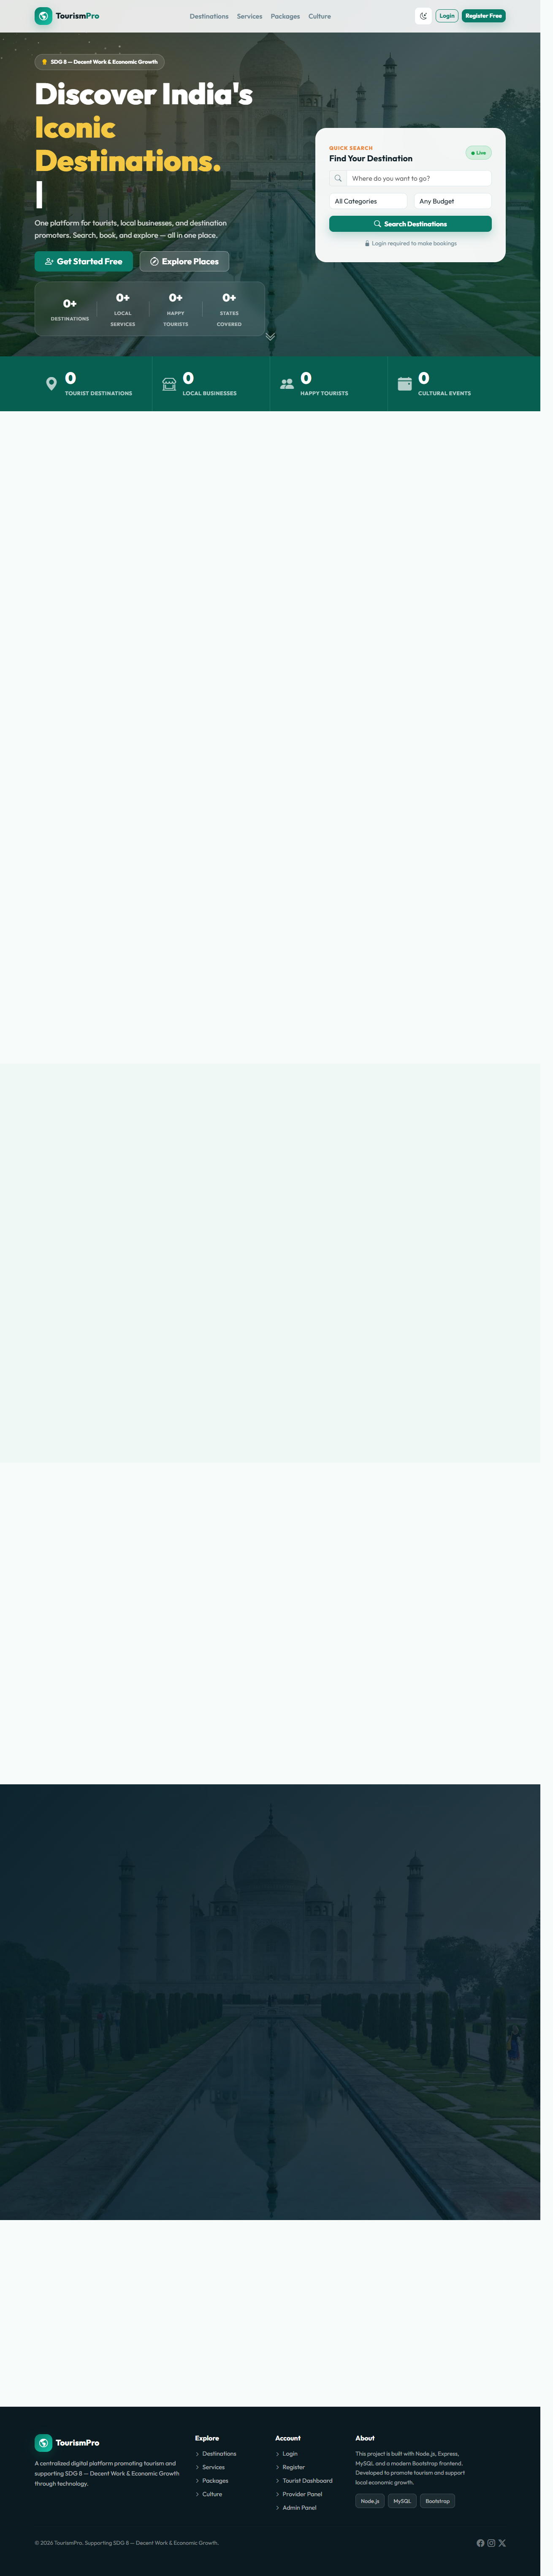
\includegraphics[width=0.95\textwidth]{landing.png}
    \caption{Landing Page -- Tourism Promotion Website}
\end{figure}

\textbf{Registration Page:}

\begin{figure}[h]
    \centering
    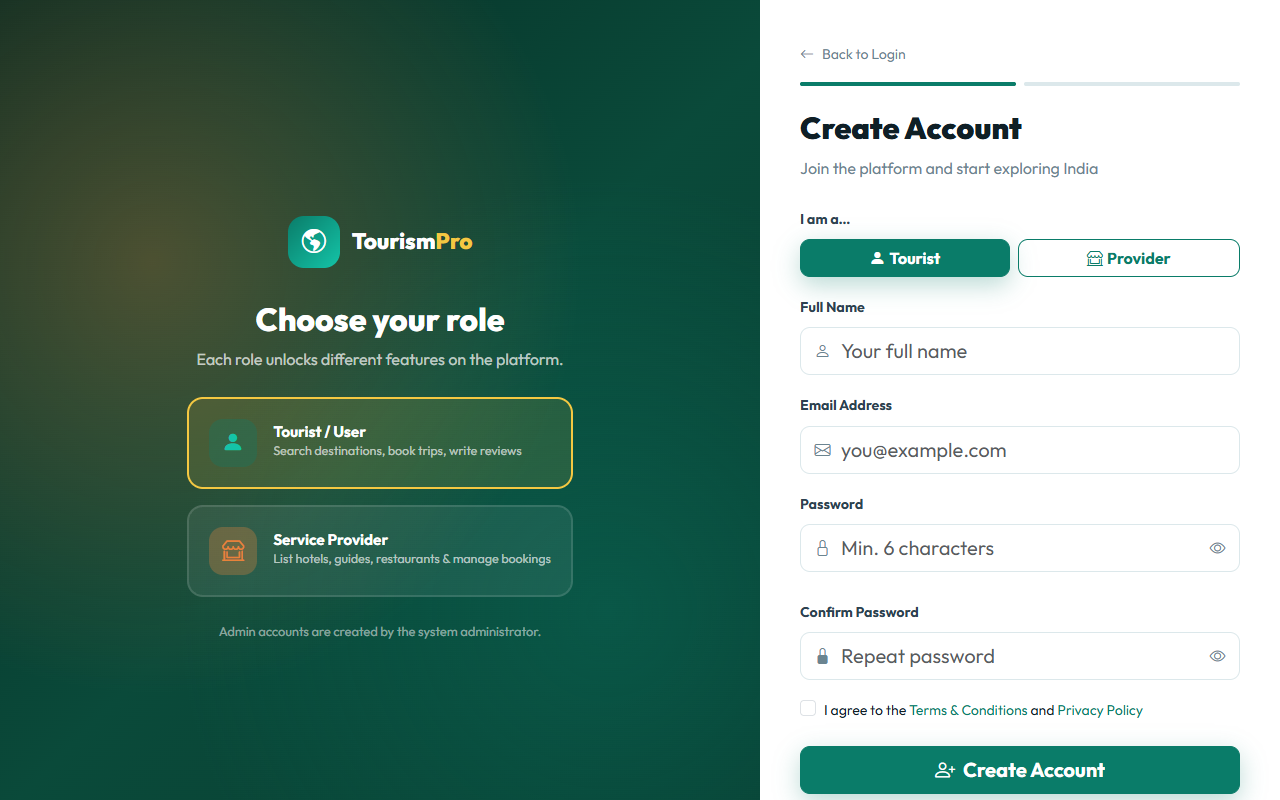
\includegraphics[width=0.95\textwidth]{register.png}
    \caption{User Registration Page}
\end{figure}

% Add more screenshots as needed:
% \begin{figure}[h]
%     \centering
%     \includegraphics[width=0.95\textwidth]{screenshots/login.png}
%     \caption{Login Page}
% \end{figure}
%
% \begin{figure}[h]
%     \centering
%     \includegraphics[width=0.95\textwidth]{screenshots/admin_dashboard.png}
%     \caption{Admin Dashboard}
% \end{figure}
%
% \begin{figure}[h]
%     \centering
%     \includegraphics[width=0.95\textwidth]{screenshots/provider_dashboard.png}
%     \caption{Service Provider Dashboard}
% \end{figure}
%
% \begin{figure}[h]
%     \centering
%     \includegraphics[width=0.95\textwidth]{screenshots/user_dashboard.png}
%     \caption{Tourist Dashboard}
% \end{figure}
%
% \begin{figure}[h]
%     \centering
%     \includegraphics[width=0.95\textwidth]{screenshots/destination_detail.png}
%     \caption{Destination Detail Page}
% \end{figure}

\section{Git Logs}

% If you have a Git repository, paste your git log output here.
% Run: git log --oneline --graph --all
% and paste the output between \begin{verbatim} and \end{verbatim}

\begin{verbatim}
commit  - Initial project setup with Express.js and MySQL
commit  - Database schema with destinations, services,
          packages, events, bookings, and reviews
commit  - Authentication system with JWT and bcrypt
commit  - Destination CRUD API routes
commit  - Booking management API
commit  - Service listing and provider API
commit  - Landing page with Bootstrap 5 and AOS animations
commit  - Login and registration pages with role selection
commit  - Admin dashboard with user and content management
commit  - Tourist dashboard with bookings and wishlists
commit  - Provider dashboard with service management
commit  - Payment processing module
commit  - Notification system implementation
commit  - Analytics dashboard for admin
commit  - Database migration v2 with extended tables
commit  - Provider approval workflow
commit  - Dark/light theme toggle
commit  - Responsive design improvements
commit  - Final testing and bug fixes
commit  - Documentation and project report
\end{verbatim}

% To generate actual git logs, run the following command
% in your project directory and replace the above:
%   git log --oneline -20


\end{document}